\newcommand{\DoNotLoadEpstopdf}{}
\documentclass[11pt]{article}
\usepackage[T1]{fontenc}
\usepackage{lmodern}
\usepackage[margin=1in]{geometry}
\usepackage{amsmath,amssymb,amsthm,mathtools}
\usepackage{enumitem,booktabs,microtype,xcolor}
\usepackage{tikz}
\usetikzlibrary{arrows.meta,positioning}
\usepackage{hyperref}
\hypersetup{pdftitle={Constant-factor hardness of directed feedback vertex set},pdfauthor={OpenAI},colorlinks=true,linkcolor=blue!50!black,citecolor=blue!50!black,urlcolor=blue!50!black}
\AddToHook{cmd/thebibliography/after}{\addcontentsline{toc}{section}{\refname}}
\ifdefined\pdftrailerid\pdftrailerid{}\fi
\newtheorem{theorem}{Theorem}[section]
\newtheorem{lemma}[theorem]{Lemma}
\newtheorem{proposition}[theorem]{Proposition}
\newtheorem{corollary}[theorem]{Corollary}
\newtheorem{claim}[theorem]{Claim}
\theoremstyle{definition}
\newtheorem{definition}[theorem]{Definition}
\theoremstyle{remark}
\newtheorem{remark}[theorem]{Remark}
\numberwithin{equation}{section}
\newcommand{\N}{\mathbb N}
\newcommand{\R}{\mathbb R}
\newcommand{\E}{\mathbb E}
\newcommand{\Prob}{\mathbb P}
\DeclareMathOperator{\DFVS}{DFVS}
\DeclareMathOperator{\TV}{TV}
\newcommand{\ind}[1]{\mathbf 1\{#1\}}
\newcommand{\abs}[1]{\lvert#1\rvert}
\newcommand{\norm}[1]{\lVert#1\rVert}
\setlist{itemsep=3pt,topsep=5pt}
\title{Constant-factor hardness of\\directed feedback vertex set}
\author{OpenAI}
\date{September 23, 2026}
\begin{document}
\maketitle
\begin{abstract}
Approximating minimum directed feedback vertex set within any fixed
constant factor is NP-hard, even on unweighted digraphs.
\end{abstract}
\tableofcontents
\section{Introduction}\label{sec:introduction}

A directed feedback vertex set of a finite digraph $G$ is a set
$F\subseteq V(G)$ for which the induced digraph $G-F$ is acyclic. Write
\[
  \DFVS(G)=\min\{\abs F:G-F\text{ is acyclic}\}.
\]
Equivalently, $F$ intersects every directed cycle. A topological order
of $G-F$ certifies this property in polynomial time. The minimum-cost
version assigns a positive rational cost to each vertex and minimizes
the sum of the deleted costs. Throughout, digraphs are finite and
loopless; two vertices may have arcs in both directions. An
$A$-approximation, for $A\ge1$, returns a feedback vertex set of
size at most $A\DFVS(G)$.

\subsection{The approximation question}

Writing $n=\abs{V(G)}$, the general $O(\log n\log\log n)$
approximation guarantee originates
in Seymour's work on fractional packing of directed circuits
\cite{Seymour1995}. Even, Naor, Schieber, and Sudan give a constructive
algorithm covering weighted directed feedback sets \cite{Even1998}.

Ordinary NP-hardness of approximation already follows from Vertex Cover,
which asks for a smallest vertex set meeting every edge of an undirected graph.
Replacing every edge of an undirected graph by its two opposite arcs
makes a vertex set a directed feedback vertex set exactly when it is a
vertex cover. Thus the earlier hardness factors below
$10\sqrt5-21$ of Dinur and Safra \cite{DinurSafra2005}, and the factors
strictly below $\sqrt2$ obtained by the completed two-to-one games line
\cite[Section~1.3.1]{KMS2018}, transfer to DFVS. These results exclude
particular constants; excluding every constant had required a stronger
complexity assumption.

Guruswami, Manokaran, and Raghavendra established
the Unique-Games barrier against every constant factor through maximum
acyclic subgraph and feedback arc set \cite{GMR2008}. The expanded
ordering-constraint framework appears in the journal paper with
H\aa stad and Charikar \cite{GHMRC2011}. Svensson gave a direct
Unique-Games-based construction with strong structure in the YES case
\cite{Svensson2013}. Guruswami and Lee subsequently gave a simpler proof
with structured completeness and short cycles in every sufficiently
large induced subgraph in the NO case \cite{GuruswamiLee2016}.
The recent discussion of Ghorbani and Mnich records the remaining gap
for general digraphs \cite{GhorbaniMnich2026}.

We prove the corresponding exclusion of every constant factor from
ordinary NP-hardness.

\begin{theorem}\label{thm:main}
For every fixed real constant $A\ge1$, it is NP-hard to approximate
minimum directed feedback vertex set within factor $A$ on unweighted
digraphs. More precisely, there is a deterministic polynomial-time
reduction from an NP-hard promise problem to instances $(G,k)$ with
$k\in\N_{>0}$. The polynomial and its constants may depend on $A$.
The reduction has the following alternatives:
\[
  \textnormal{YES: }\DFVS(G)\le k,
  \qquad
  \textnormal{NO: }\DFVS(G)>Ak.
\]
\end{theorem}

Theorem~\ref{thm:main} implies that a deterministic polynomial-time
algorithm with any constant approximation guarantee exists if and
only if $\mathrm P=\mathrm{NP}$. For the reverse implication, membership
of the size-bounded decision problem in NP permits exact optimization
and witness search when $\mathrm P=\mathrm{NP}$. The theorem establishes
that the required approximation factor grows without bound with the
input size, assuming $\mathrm P\ne\mathrm{NP}$. It does not identify
that growth rate or improve the general approximation algorithm.

A directed feedback arc set is a set of arcs whose deletion leaves an
acyclic digraph. Corollary~\ref{cor:feedback-arc} transfers the same
hardness to this problem on unweighted simple loopless digraphs, through
a reduction preserving both the optimum and approximation solutions.
The vertex-set hardness also holds when opposite arcs are forbidden,
as shown in Remark~\ref{rem:no-opposite-arcs}.

\subsection{Methodological background}

Our construction shares the useful division between protected vertices
and deletable test vertices in Svensson's dictatorship gadget
\cite[Section~3.1.1]{Svensson2013}. His soundness proof also reads a
Boolean function from a topological order
\cite[Section~3.1.3]{Svensson2013}. Here the protected vertices encode
rank profiles, and compatibility across tuple prefixes supplies a
family of monotone functions. Svensson uses the ``It Ain't Over Till
It's Over'' theorem; Guruswami and Lee instead use an invariance
principle \cite[Section~1]{GuruswamiLee2016}. Our analytic input is
Friedgut's theorem on Boolean functions of bounded total influence
\cite{Friedgut1998}. We derive its required fixed-bias form explicitly.
Junta-based label decoding already appears in Dinur and Safra's
Vertex Cover hardness proof \cite[Sections~1.1 and~3]{DinurSafra2005},
where a nearby bias is selected to obtain bounded total influence.
Here a single pivotality budget controls all the prescribed biases,
and the contradiction requires their estimates to concern the same
distribution of functions.

The rank distribution is obtained by combining finite Ramsey theory
\cite{Ramsey1930} with finite minimax \cite{vonNeumann1928}.
These are the external combinatorial tools in the rank-spreading
argument. The shared-prefix construction and the permutation
pivotality budget are proved below. Their role is to compare many
biases without changing the distribution of the functions being
analyzed. The source of hardness is the published imperfect-completeness
two-to-one theorem, so the proof does not consume a Unique Games
hardness theorem.

\subsection{The reduction and its new ingredients}

A two-to-one game has a bipartite constraint graph with a label set
$X$ at each big-side vertex and a label set $Y$ at each small-side
vertex. Each edge carries a map $X\to Y$ with exactly two preimages
per label; an edge is satisfied when the chosen endpoint labels obey
that map. The game value is the largest fraction of satisfied edges,
measured under its prescribed edge distribution.
Our starting point is the imperfect-completeness 2-to-1 Games Theorem,
obtained through the work of Dinur, Khot, Kindler, Minzer, and Safra,
Khot, Minzer, and Safra, and Barak, Kothari, and Steurer
\cite{DKKMS2025,KMS2018,BKS2019}. We use its precise form in
Theorem~\ref{thm:games}: for arbitrarily small constant $\theta>0$,
distinguishing game value at least $1-\theta$ from value at most
$\theta$ is NP-hard, with fixed alphabets and exact two-element
projection fibers. The perfect-completeness 2-to-1 Games Conjecture
is not a premise of the argument.

The central difficulty is to extract a game labeling from an arbitrary
acyclic remainder. An acyclic graph supplies a topological order, but
its order can interleave the many vertices representing the same local
test. The proof first makes comparisons within that order consistent,
then interprets them as Boolean functions. Small deletion cost will
constrain these functions in incompatible ways.

For a fixed integer factor $A$, put $D=10A$. We construct a weighted
graph with a feedback vertex set of cost at most $4$ in the YES case.
Suppose, toward the soundness contradiction, that a NO instance has
one of cost at most $D$. Fix a topological order after its deletion.
The following four steps analyze this arbitrary order. A Boolean
function on subsets is evaluated at bias $p$ by including each label
independently with probability $p$; its acceptance is the probability
that its value is one.

\begin{enumerate}[label=\textup{(\arabic*)}]
\item \emph{Rank comparisons with a common interpretation.}
For each short tuple of game vertices, we create vertices indexed by
rank-valued functions of label tuples. A global labeling evaluates
all these functions consistently. In the soundness analysis, a
putative inexpensive feedback set leaves every rank vertex present,
so its surviving topological order supplies comparison bits. A
finite Ramsey and minimax argument produces a distribution on rank
embeddings for which all triples of positions have nearly identical
image laws. Ordered comparisons then agree with high probability,
yielding a monotone Boolean function of subsets of label tuples.

\item \emph{Conditioning through a shared prefix.}
Successive random subsets split label tuples into lexicographically
ordered cells. Monotonicity selects a unique transition cell, and
prefix identifications make these transitions consistent under
refinement. A full-prefix test prevents the chosen cell from having
too few membership-one steps at any of many dyadic biases. On
averaging, the conditioned big-side Boolean function has acceptance
at least a constant multiple of the bias at every scale. The same
prefix data define functions for every game vertex before a fresh
constraint is drawn.

\item \emph{A pivotality budget independent of the alphabet size.}
A single-label test charges the event that the starred label can be
pivotal somewhere along a random permutation. The resulting quantity $B(f)$ is the sum, over labels, of the
probability that the label is pivotal at some prefix of a random
permutation of the other labels. It bounds both total influence and
acceptance probability divided by the bias, at every bias. Its
expectation is at most $D+1$ on either side of the game. Friedgut's junta theorem \cite{Friedgut1998}, transferred
to fixed dyadic biases, therefore supplies bounded coordinate lists
outside a small exceptional set. Their size is fixed before choosing
the game alphabets.

\item \emph{A common tail variable across all scales.}
A projection-respecting coupling compares bias $p$ on the big side
with bias $2p$ on the small side. Game soundness makes the two junta
lists typically use disjoint projection fibers. The corresponding
outputs are then independent under the coupling, allowing the
comparison bound to pass to product measures. At each dyadic bias, this forces a positive contribution of constant
size to the tail sum of the small-side pivotality budget. All these
estimates concern the same random variable under the same distribution.
Adding sufficiently many such contributions contradicts its expected
budget.
\end{enumerate}

The pivotality quantity is independent of the bias. This is essential:
a separate influence bound at each scale would not justify adding the
contributions to one tail sum. Likewise, the shared prefix fixes all
vertex functions before the tested game edge is drawn; otherwise the
coordinate lists would not define a game labeling.

The proof uses finite probability spaces to specify weighted test
families. Every outcome is included explicitly with its probability
as part of its cost. Thus the reduction is deterministic. All
parameters, alphabets, tuple lengths, and rank tables are constants
once the target factor is fixed, even though some are extremely
large. Finally, rounding each vertex cost upward and replacing a
vertex by an independent cluster produces an unweighted gap.

\subsection{Organization}

Section~\ref{sec:preliminaries} states the external theorems and proves
the required dyadic junta corollary.
Section~\ref{sec:construction} gives the parameter choices, graph,
tests, and completeness argument. Section~\ref{sec:ranks} proves rank
spreading and the order lemmas used to read Boolean functions from a
surviving graph. Sections~\ref{sec:prefix} and~\ref{sec:pivotality}
establish the acceptance lower bounds and pivotality budgets.
Section~\ref{sec:soundness} gives the comparison and tail-sum
contradiction. Section~\ref{sec:unweighting} removes the costs and
proves Theorem~\ref{thm:main}.

\section{Games and Boolean functions}
\label{sec:preliminaries}

For a finite set \(S\), we identify \(\{0,1\}^{S}\) with the power set
\(2^{S}\).  For \(p\in(0,1)\), let \(\mu_p^{S}\) be the probability
measure on \(2^{S}\) in which each element belongs to the sampled set
independently with probability \(p\).  We use \([n]=\{1,\ldots,n\}\).
All graphs and probability spaces in the reduction are finite.

\subsection{The game used in the reduction}

A two-to-one game consists of a bipartite constraint graph with disjoint
vertex sets \(U,V\), nonempty label sets \(X,Y\) with
\(\abs{X}=2\abs{Y}\), and, for each edge \(e=(u,v)\), a map
\(\pi_e:X\to Y\) for which every fiber has cardinality two.  Parallel
constraints are allowed.  The edges carry a rational probability
distribution \(\nu\).  Its endpoint marginals are denoted by
\(\nu_U\) and \(\nu_V\).  A labeling consists of maps
\(\ell_U:U\to X\) and \(\ell_V:V\to Y\); its value is
\[
  \Pr_{e=(u,v)\sim\nu}
  [\,\pi_e(\ell_U(u))=\ell_V(v)\,].
\]
The value of a game is the maximum of this expression over all
labelings.

\begin{theorem}[Two-to-one games with imperfect completeness]
\label{thm:games}
For every constant \(\theta\in(0,1/2)\), there are constant label
sets \(X,Y\) such that it is \(\mathrm{NP}\)-hard, by a deterministic
polynomial-time reduction, to distinguish two-to-one games of the
following kinds:
\begin{enumerate}[label=\textup{(\roman*)}]
  \item there is a labeling of value at least \(1-\theta\);
  \item every labeling has value at most \(\theta\).
\end{enumerate}
Every constraint is a total map \(X\to Y\) with exactly two preimages
of each label in \(Y\).  The label sets may depend on \(\theta\).
\end{theorem}

We invoke the completed theorem in this precise form.
Dinur, Khot, Kindler, Minzer, and Safra prove the stated gap
conditionally on their Grassmann agreement hypothesis
\cite[Theorem~1.8]{DKKMS2025}.  Their Hypothesis~3.6 follows from the
Grassmann expansion theorem of Khot, Minzer, and Safra
\cite[Theorem~1.12, ECCC revision~2]{KMS2018} through the implications
of Barak, Kothari, and Steurer
\cite[Section~1.1 and Theorems~9--11]{BKS2019}.
The two-to-one definition and the common alphabets are as in
\cite[Definitions~1.1--1.2 and Section~4.2]{DKKMS2025}.
In the explicit constraint construction, the smoothing parameter may
be chosen rational within its permitted range
\cite[Sections~4.2 and~5.2]{DKKMS2025}. The edge sampling process then
specifies rational weights: all constant-length tuples and constant-dimensional
subspaces can be enumerated, followed by the prescribed identifications.
With the parameters fixed, this is a deterministic finite construction
of polynomial size.  Thus the use of a rational edge law does not
introduce randomness into the reduction.  We require neither perfect
completeness nor any degree regularity of the game.

\subsection{Junta approximation at fixed dyadic biases}

For a Boolean function \(f:2^S\to\{0,1\}\) and \(j\in S\), define
\begin{equation}
\label{eq:biased-influence}
  I_{p,j}(f)
  =\Pr_{R\sim\mu_p^{S\setminus\{j\}}}
       [\,f(R)\ne f(R\cup\{j\})\,],
  \qquad
  I_p(f)=\sum_{j\in S} I_{p,j}(f).
\end{equation}
This is also the probability that flipping coordinate \(j\) changes
the value of \(f\), when the entire input has law \(\mu_p^S\):
the change event depends only on the other coordinates.
A function is a \emph{junta on \(J\subseteq S\)} if its value depends
only on \(R\cap J\).  Constant functions are juntas on the empty set.

\begin{theorem}[Friedgut's junta theorem]
\label{thm:friedgut}
For every \(b\ge0\) and \(\alpha>0\), there is a finite integer
\(J_{\mathrm{unif}}(b,\alpha)\) with the following property.
For every finite \(S\) and every Boolean function
\(f:2^S\to\{0,1\}\) with \(I_{1/2}(f)\le b\), there is a Boolean
function \(\widetilde f\), depending on at most
\(J_{\mathrm{unif}}(b,\alpha)\) coordinates, for which
\[
  \Pr_{R\sim\mu_{1/2}^{S}}[\,f(R)\ne\widetilde f(R)\,]\le\alpha.
\]
The bound is independent of \(\abs S\).
\end{theorem}

This is the uniform version of Friedgut's theorem
\cite[Theorem~1.1 in the February 3, 1998 author manuscript]{Friedgut1998}.
Friedgut also proves a biased-product version
\cite[Theorem~4.1 in the same manuscript]{Friedgut1998}.
We give an elementary reduction of the dyadic case to the uniform case,
so that the dependence on the bias and independence of the game
alphabet size are explicit.

\begin{corollary}[Dyadic junta approximation]
\label{cor:dyadic-junta}
Let \(p=2^{-k}\), where \(k\ge1\) is an integer.  For every \(b\ge0\)
and \(\alpha>0\), there is a finite integer \(J(p,b,\alpha)\),
independent of \(\abs S\), such that every Boolean function
\(f:2^S\to\{0,1\}\) with \(I_p(f)\le b\) has a Boolean junta
approximant on at most \(J(p,b,\alpha)\) coordinates with error at
most \(\alpha\) under \(\mu_p^S\).
\end{corollary}

\begin{proof}
The assertion is immediate for \(S=\varnothing\), so assume otherwise.
Let \((X_{j,a})_{j\in S,\,a\in[k]}\) be independent uniform bits and
put
\[
  Z_j=\bigwedge_{a=1}^k X_{j,a},
  \qquad
  F(X)=f(\{j\in S:Z_j=1\}).
\]
The \(Z_j\) are independent Bernoulli \(p\) bits.  Flipping \(X_{j,a}\)
changes \(F\) precisely when all the other \(k-1\) bits of its block
are one and coordinate \(j\) is pivotal for the values of the other
blocks.  These two events are independent.  Therefore
\begin{equation}
\label{eq:and-block-influence}
  I_{1/2}(F)
   =k2^{-(k-1)}I_p(f)
   =2kpI_p(f)
   \le kb.
\end{equation}
By Theorem~\ref{thm:friedgut}, there is a Boolean approximant \(H\)
to \(F\) with error at most \(\alpha\), using at most
\(J_{\mathrm{unif}}(kb,\alpha)\) of the individual bits \(X_{j,a}\).
Let \(J\subseteq S\) be the set of blocks touched by these bits.
Then \(\abs J\le J_{\mathrm{unif}}(kb,\alpha)\).

Reveal all bits in every block indexed by \(J\).  Since \(H\) is
measurable with respect to these revealed blocks, the Boolean
predictor with smallest conditional error from the revealed blocks
has total error at most that of \(H\).  More explicitly, this
predictor outputs one when the conditional probability of \(F=1\)
is at least \(1/2\), with any fixed convention at equality.
The unrevealed blocks remain independent of the revealed blocks,
and the dependence of \(F\) on a revealed block is only through its
AND value.  Consequently
\[
 \Pr[\,F=1\mid (X_{j,a})_{j\in J,\,a\in[k]}\,]
 =
 \Pr[\,f(\{j:Z_j=1\})=1\mid (Z_j)_{j\in J}\,].
\]
The optimal predictor is therefore a Boolean function only of
\((Z_j)_{j\in J}\).  Regard it as a function
\(\widetilde f:2^S\to\{0,1\}\) on the original coordinates.
The induced law of the original input is \(\mu_p^S\), so
\[
  \Pr_{R\sim\mu_p^S}[\,f(R)\ne\widetilde f(R)\,]\le\alpha.
\]
Thus \(J(p,b,\alpha)=J_{\mathrm{unif}}(kb,\alpha)\) is a valid
choice, increased to one if desired.
\end{proof}

\begin{remark}
The junta approximants need not be monotone.  In the reduction, the
original conditioned functions will be monotone, but the argument
uses only their approximation errors and their coordinate supports.
For any fixed finite collection of dyadic biases, the maximum of the
bounds in Corollary~\ref{cor:dyadic-junta} remains independent of the
alphabet size.
\end{remark}

\section{The weighted reduction}
\label{sec:construction}

We first construct a digraph with positive rational vertex costs.  Write
$w_v$ for the cost of a vertex $v$ and $w(F)=\sum_{v\in F}w_v$ for the cost
of a vertex set $F$.  For each
fixed integer $A\ge 1$, the construction will have a feedback vertex set of
cost at most $4$ in the completeness case of Theorem~\ref{thm:games}, whereas
every feedback vertex set will have cost greater than $D=10A$ in its soundness
case.  Section~\ref{sec:unweighting} converts this gap into an unweighted one.

\subsection{Choice of parameters}
\label{sec:parameters}

Fix an integer $A\ge 1$ and put $D=10A$. The constants have the following
roles. There will be $M$ bias scales and at most $T$ prefix slots.
The full-prefix and comparison tests have total costs $H$ and $K$.
The junta size is bounded by $J$, independently of the game alphabets;
$\theta$ is the required game accuracy. Finally $L$ and $N$ specify
finite ordered rank sets, and $\psi:[L]\hookrightarrow[N]$ is an
increasing random embedding. Its purpose is to make the order
comparisons insensitive to their precise rank levels, as proved in
Lemma~\ref{lem:rank-spreading}.
Choose the constants in the following order.
\begin{enumerate}[label=\arabic*.]
  \item Set
  \[
    M=128(D+1),\qquad
    p_i=2^{-(i+1)},\qquad q_i=2p_i\quad (i\in[M]),
    \qquad \gamma=\frac{p_M}{1000}.
  \]
  \item Set $H=8(D+1)$.  Choose an integer $T\ge 1$ large enough that
  \begin{equation}
    HM\exp\left(-\frac{p_MT}{8M}\right)\le 1,
    \label{eq:prefix-length-choice}
  \end{equation}
  and an integer
  \begin{equation}
    K\ge \frac{M2^T D}{\gamma}.
    \label{eq:comparison-mass-choice}
  \end{equation}
  \item Put $B_0=(D+1)/\gamma$.  By Corollary~\ref{cor:dyadic-junta}, there
  is an integer $J\ge 1$ that bounds the size of a junta approximant with
  error at most $\gamma$ for every function of total influence at most $B_0$
  at any of the biases $p_i,q_i$, $i\in[M]$.  Choose a positive rational
  $\theta$ small enough that Theorem~\ref{thm:games} applies and
  \begin{equation}
    K\theta\le 1,\qquad J^2\theta\le\gamma.
    \label{eq:game-accuracy-choice}
  \end{equation}
  Apply that theorem with this fixed $\theta$, and let $X,Y$ be its
  alphabets, with $m=\abs{X}=2\abs{Y}$.
  \item Put
  \[
    k_{\max}=2^Tm,\qquad L=10k_{\max}+30,
    \qquad \rho=\min\{\gamma,1/m\}.
  \]
  Choose a positive rational $\eta$ satisfying
  \begin{equation}
    3\eta L^3 2^{m^T}\le\rho.
    \label{eq:rank-accuracy-choice}
  \end{equation}
  Apply Lemma~\ref{lem:rank-spreading} to $L,\eta$, obtaining a finite $N$
  and a rational probability distribution on increasing maps
  $\psi:[L]\hookrightarrow[N]$.  Fix this distribution for the construction.
\end{enumerate}

All these quantities depend only on $A$.  In particular, the junta bound
$J$ is fixed \emph{before} the alphabet size $m$ is determined.  Its existence
does not require an alphabet bound.  The later choices of $\rho,\eta,N$
therefore introduce no dependence back into the choice of $\theta$.

Let the input game have bipartition $U,V$, edge distribution $\nu$, and
endpoint marginals $\nu_U,\nu_V$.  For an edge $e=(u,v)$, write
$\pi_e:X\to Y$ for its two-to-one projection.  All probability distributions
below are finite and rational.  A sampling description specifies a separate
vertex for each outcome of positive probability, with the indicated
probability as a factor in its cost.  The reduction enumerates these outcomes;
it does not sample a random output graph.

\subsection{Rank vertices and their identifications}

\begin{definition}[Rank graph]
\label{def:rank-graph}
For $w\in U\cup V$, let $\Lambda_w=X$ if $w\in U$ and $\Lambda_w=Y$ if
$w\in V$, and put $m_w=\abs{\Lambda_w}$.  The allowed vertex tuples are
\[
  \bigcup_{t=0}^{T}U^t
  \quad\cup\quad
  \bigcup_{t=0}^{T-1}(U^t\times V).
\]
Tuples are ordered sequences and may contain repeated vertices.  For an
allowed tuple $\mathbf d=(w_1,\ldots,w_t)$, let
$\Lambda_{\mathbf d}=\prod_{j=1}^t\Lambda_{w_j}$; the product for the empty
tuple is a singleton.  In every case
\begin{equation}
  \abs{\Lambda_{\mathbf d}}\le m^T.
  \label{eq:tuple-domain-bound}
\end{equation}
For every function $x:\Lambda_{\mathbf d}\to[N]$, introduce a formal rank
vertex $b_{\mathbf d}(x)$.  Within each tuple, introduce an arc
$b_{\mathbf d}(x)\to b_{\mathbf d}(y)$ whenever
\[
  x(\lambda)<y(\lambda)
  \qquad\text{for every }\lambda\in\Lambda_{\mathbf d}.
\]
Whenever $\mathbf s w$ is an allowed extension of $\mathbf s$, identify
\begin{equation}
  b_{\mathbf s}(x)
  \equiv b_{\mathbf s w}(x\circ\operatorname{proj}),
  \label{eq:prefix-identification}
\end{equation}
where $\operatorname{proj}:\Lambda_{\mathbf s w}\to\Lambda_{\mathbf s}$
drops the last coordinate.  Take the equivalence relation generated by all
these identifications and keep the induced arcs between its classes.  Each
resulting rank vertex has cost $D+1$, independently of the number of its
formal representatives.  We use the same notation for a formal vertex and
its equivalence class.  The vertices represented by the constant profiles
with value $j$ are denoted by $o_j$, for $j\in[N]$.
\end{definition}

\begin{lemma}[Evaluation invariant]
\label{lem:evaluation-invariant}
Every global game labeling $\ell$ gives a well-defined real value on the
rank vertices by
\[
  b_{\mathbf d}(x)\longmapsto x(\ell(\mathbf d)),
\]
where $\ell(\mathbf d)$ is the tuple of labels supplied by $\ell$.  Every
rank arc strictly increases this value.  Consequently, the rank graph has
no self-loops, and $o_1,\ldots,o_N$ are distinct vertices with an arc
$o_j\to o_{j'}$ whenever $j<j'$.
\end{lemma}

\begin{proof}
For every generating identification in
Equation~\eqref{eq:prefix-identification},
\[
  (x\circ\operatorname{proj})(\ell(\mathbf s),\ell(w))
  =x(\ell(\mathbf s)).
\]
Thus evaluation is constant on each equivalence class.  This remains true
when vertices repeat in a tuple: their repeated coordinates are evaluated
at the same global label.  A rank arc is strictly increasing at every tuple
of labels, and hence at the particular tuple supplied by $\ell$.  Its two
endpoints cannot become the same equivalence class.  Finally, constant
profiles all identify with their representatives at the empty tuple, and
their evaluated values are the distinct integers $1,\ldots,N$.
\end{proof}

This division into protected rank vertices and deletable tests is related
to the bit-vertex/test-vertex architecture of
\cite[Section~3.1.1]{Svensson2013}; here the rank profiles and prefix
identifications enforce the consistency needed below.
All other vertices will be test vertices, distinct from the rank vertices
and from one another.  Their arcs will be incident only to rank vertices.
For $E\subseteq\Lambda_{\mathbf d}$ and $1\le a<h\le L$, write
\[
  b_{\mathbf d}^{\psi}(E;a,h)=b_{\mathbf d}(x),\qquad
  x(\lambda)=
  \begin{cases}
    \psi(a),&\lambda\in E,\\
    \psi(h),&\lambda\notin E.
  \end{cases}
\]

\subsection{Wildcard vertices and prefix data}

\begin{definition}[Wildcard vertex]
\label{def:wildcard}
Fix an allowed tuple $\mathbf d$, an increasing map $\psi$, an ordered
partition $C_1,\ldots,C_k$ of $\Lambda_{\mathbf d}$ with
$1\le k\le k_{\max}$, and a set $Z\subseteq\Lambda_{\mathbf d}$, called
the star set.  Empty cells in the partition are permitted.  Put
$z_\ell=\psi(10\ell+10)$ for $\ell\in[k]$.  The corresponding wildcard
vertex has an incoming arc from every rank vertex $b_{\mathbf d}(x)$ for
which
\begin{equation}
  x(\lambda)<z_\ell
  \quad\text{for all }\ell\in[k]
  \text{ and }\lambda\in C_\ell\setminus Z,
  \label{eq:wildcard-incoming}
\end{equation}
and an outgoing arc to every $b_{\mathbf d}(x)$ satisfying the strict
reverse inequalities
\begin{equation}
  x(\lambda)>z_\ell
  \quad\text{for all }\ell\in[k]
  \text{ and }\lambda\in C_\ell\setminus Z.
  \label{eq:wildcard-outgoing}
\end{equation}
There are no restrictions on the values of $x$ on $Z$.
\end{definition}

The wildcard inequalities have a direct interpretation under any global
labeling. If its evaluated tuple lies in $C_r\setminus Z$, the threshold
$z_r$ lies strictly between the evaluations of every incoming and every
outgoing rank vertex. Assigning that threshold to the test therefore extends
the increasing evaluation along its incident arcs. At starred tuples, the
arc conditions impose no restriction on these evaluated values; the
completeness argument will delete the corresponding test.

\begin{definition}[Prefix data]
\label{def:prefix-data}
For $t\in\{0,\ldots,T\}$, draw
$\mathbf s=(u_1,\ldots,u_t)$ independently from $\nu_U$ in each slot.
Independently draw $i_1,\ldots,i_t$ uniformly from $[M]$.  Conditional on
these indices, draw $P_j\subseteq X$ using independent Bernoulli
$p_{i_j}$ membership bits, independently for different slots $j$.
Partition $\Lambda_{\mathbf s}$ by the membership patterns
\[
  \bigl(\ind{\lambda_j\in P_j}\bigr)_{j=1}^t,
  \qquad \lambda\in\Lambda_{\mathbf s}.
\]
Order the $2^t$ cells lexicographically with $1$ before $0$, keeping cells
that happen to be empty, and denote them by $C_1,\ldots,C_{2^t}$.  Put
\[
  C_{<r}=\bigcup_{\ell<r}C_\ell,
  \qquad C_{\le r}=\bigcup_{\ell\le r}C_\ell.
\]
At $t=0$ this is the one-cell partition of the singleton product domain.
\end{definition}

\subsection{The three test families}

\begin{definition}[Test families]
\label{def:tests}
Add the following families of test vertices to the rank graph.  In each
family, independently draw $\psi$ from the fixed rank distribution.  Each
outcome is a separate vertex with cost equal to its probability multiplied
by the stated total mass.  Distinct outcomes remain separate even if they
produce the same incident arcs.
\begin{enumerate}[label=\arabic*.,leftmargin=*]
  \item \textbf{Full-prefix tests, of total mass $H$.}
  \label{item:full-prefix-test}
  Draw prefix data at length $T$ and use the wildcard vertex in tuple
  $\mathbf s$ with those $2^T$ cells.  Its star set is
  \begin{equation}
    Z=\left\{\lambda\in\Lambda_{\mathbf s}:
      \text{there exists }i\in[M]\text{ such that }
      \#\{j:i_j=i,\ \lambda_j\in P_j\}
      <\frac{p_iT}{2M}\right\}.
    \label{eq:full-prefix-stars}
  \end{equation}

  \item \textbf{Single-label tests, with one family on each side.}
  \label{item:single-label-test}
  The big-side family has total mass $\abs{X}$, and the small-side family
  has total mass $\abs{Y}$.  Choose $t$ uniformly from
  $\{0,\ldots,T-1\}$ and draw prefix data at length $t$.  Independently
  draw $w$ from the endpoint marginal on the chosen side, a uniformly
  random label $j_0\in\Lambda_w$, and a uniformly random permutation
  $(\sigma(1),\ldots,\sigma(m_w))$ of $\Lambda_w$.  Use a wildcard vertex
  in tuple $\mathbf s w$.  Its cells, in order, are
  \[
    C_\ell\times\{\sigma(a)\},
    \qquad \ell=1,\ldots,2^t,\quad a=1,\ldots,m_w,
  \]
  with the prefix-cell index first.  Thus the same label permutation is
  used in every prefix cell.  Its star set is
  $Z=\Lambda_{\mathbf s}\times\{j_0\}$.

  \item \textbf{Comparison tests, of total mass $K$.}
  \label{item:comparison-test}
  Choose $t$ uniformly from $\{0,\ldots,T-1\}$ and draw prefix data at
  that length.  Independently draw an edge $e=(u,v)$ from $\nu$ and an
  index $i$ uniformly from $[M]$.  Conditional on $t$, choose $r$ uniformly
  from $[2^t]$, independently of all other choices.

  Draw $R_u\subseteq X$ and $R_v\subseteq Y$ by the following coupling.
  Independently in each block indexed by $y\in Y$, draw the two bits on
  $\pi_e^{-1}(y)$ independently with probability $p_i$ of being one.  If
  either is one, set the bit at $y$ to one.  If both are zero, set it to
  one with probability
  \begin{equation}
    \frac{p_i^2}{(1-p_i)^2}.
    \label{eq:coupling-residual}
  \end{equation}
  This is a valid probability because $p_i\le 1/4$.  The marginal
  probability of the bit at $y$ being one is
  \[
    1-(1-p_i)^2+(1-p_i)^2\frac{p_i^2}{(1-p_i)^2}
    =2p_i=q_i.
  \]
  Hence the two complete marginals are the product measures of biases
  $p_i$ and $q_i$, respectively.  Different projection blocks are
  independent, and
  \begin{equation}
    R_u\subseteq\pi_e^{-1}(R_v)
    \label{eq:coupling-inclusion}
  \end{equation}
  holds for every outcome.  These bits are fresh, independent of the
  prefix subsets.

  For $w\in\{u,v\}$ and $R\subseteq\Lambda_w$, define
  \begin{equation}
    E_w^r(R)=
      (C_{<r}\times\Lambda_w)\cup(C_r\times R).
    \label{eq:comparison-sets}
  \end{equation}
  The test vertex has just the incoming and outgoing arcs in the path
  \begin{equation}
    b_{\mathbf s v}^{\psi}(E_v^r(R_v);2,17)
    \ \longrightarrow\ \text{test}\ \longrightarrow\
    b_{\mathbf s u}^{\psi}(E_u^r(R_u);3,18).
    \label{eq:comparison-path}
  \end{equation}
\end{enumerate}
\end{definition}

All wildcard partitions have admissible size: the full-prefix family has
$2^T\le k_{\max}$ cells, and a single-label test has
$2^tm_w\le 2^{T-1}m\le k_{\max}$ cells.  Their tuples, as well as both
tuples in a comparison test, are among those of
Definition~\ref{def:rank-graph}.  The padding in $L$ contains every rank
index used above.

\subsection{Completeness}

\begin{proposition}
\label{prop:completeness}
If the input game has a labeling satisfying a fraction at least $1-\theta$
of its constraints under $\nu$, then the constructed digraph has a
feedback vertex set of cost at most $4$.
\end{proposition}

\begin{proof}
Fix such a labeling $\ell$.  Delete each wildcard test whose evaluated
tuple $\ell(\mathbf d)$ lies in its star set, and each comparison test
whose edge is not satisfied by $\ell$.  Denote this deletion set by
$F_{\mathrm{yes}}$.  No rank vertex is deleted.

We first bound its cost.  In a full-prefix test, conditional on any fixed
vertex tuple $\mathbf s$, the count
\[
  \#\{j:i_j=i,\ \ell(u_j)\in P_j\}
\]
is binomial with mean $\mu_i=p_iT/M$.  Indeed, indices and subsets are
independent between slots, so every slot contributes an independent
Bernoulli variable of parameter $p_i/M$.  This argument also applies
when the same game vertex appears in several slots.  For a binomial random
variable $Z$ of mean $\mu$, the exponential Markov inequality gives
\[
  \Pr[Z<\mu/2]
  \le e^{\mu/2}\E[e^{-Z}]
  \le\exp\bigl(-(1/2-e^{-1})\mu\bigr)
  \le\exp(-\mu/8).
\]
Here the middle inequality follows by writing
$\E[e^{-Z}]=(1-a+ae^{-1})^T\le\exp(-Ta(1-e^{-1}))$
when $Z$ has parameters $T,a$.  Applying this bound to each scale and
taking a union bound over $i\in[M]$, the deletion probability for a
full-prefix test is at most
\[
  \sum_{i=1}^{M}\exp(-\mu_i/8)
  \le M\exp\left(-\frac{p_MT}{8M}\right).
\]
After multiplication by the mass $H$, this is at most one by
Equation~\eqref{eq:prefix-length-choice}.  In a single-label test, membership
of the evaluated tuple in the star set is precisely the event
$j_0=\ell(w)$.  Its probability is $1/m_w$, so each of the two families
contributes cost one.  Comparison tests are deleted with probability at
most $\theta$, and hence contribute at most $K\theta\le1$ by
Equation~\eqref{eq:game-accuracy-choice}.  Thus
\[
  w(F_{\mathrm{yes}})\le 1+1+1+1=4.
\]

To prove that this deletion set is a feedback vertex set, assign to each
rank vertex its evaluation under $\ell$, as in
Lemma~\ref{lem:evaluation-invariant}.  Every rank arc strictly increases
the assigned value.  For a retained wildcard vertex, let $C_r$ be the
cell containing its evaluated tuple and assign the test value $z_r$.
The evaluated tuple is outside the star set.  Thus
Equations~\eqref{eq:wildcard-incoming} and~\eqref{eq:wildcard-outgoing}, at that
tuple, put every incoming rank value strictly below $z_r$ and every
outgoing rank value strictly above it.

For a retained comparison, the evaluated prefix is the same on both
sides and $\pi_e(\ell(u))=\ell(v)$.  By
Equation~\eqref{eq:coupling-inclusion},
\[
  \ell(\mathbf s u)\in E_u^r(R_u)
  \quad\Longrightarrow\quad
  \ell(\mathbf s v)\in E_v^r(R_v).
\]
The possible pairs of rank indices at the start and end of
Equation~\eqref{eq:comparison-path} are therefore $(2,3)$, $(2,18)$, and
$(17,18)$.  Each is increasing, so the corresponding evaluated values are
strictly increasing as well.  Assign this test any real value strictly
between its two endpoint values.

These assignments coexist because there are no arcs between test vertices.
Every arc remaining after deletion of $F_{\mathrm{yes}}$ strictly
increases the assigned real value.  A directed cycle would force a strict
increase back to its starting value, which is impossible.  Thus the
remaining digraph is acyclic.
\end{proof}

\subsection{Deterministic implementation}

\begin{proposition}[Deterministic polynomial construction]
\label{prop:polynomial}
For each fixed $A$, the preceding construction produces a loopless digraph
with positive rational vertex costs in deterministic polynomial time in the
game input size.  Its vertex costs are bounded above by a constant depending
only on $A$.
\end{proposition}

\begin{proof}
Put $n=1+\abs{U}+\abs{V}+\abs{E}$, counting parallel constraints as
distinct edges if necessary.  The number of allowed tuples is at most
$(2T+1)n^T$.  By Equation~\eqref{eq:tuple-domain-bound}, a tuple has at most
$N^{m^T}$ formal rank vertices.  Both factors other than $n^T$ are constants
for fixed $A$.

For each slot, there are at most $M2^m$ choices of index and subset.  The
support of the rank law, the number of permutations of either alphabet,
and all choices of individual labels are also bounded by constants.  A
full-prefix test uses $T$ game-vertex slots, so this family has
$O_A(n^T)$ outcomes.  A single-label test has at most $T-1$ prefix vertices and one
endpoint, again giving $O_A(n^T)$ outcomes.  A comparison test has at most
$T-1$ prefix vertices and one input edge; its remaining choices, including
the coupled subsets and candidate cell, range over constant finite sets.
Thus there are $O_A(n^T)$ comparison outcomes as well.  Here $O_A$ allows
the implicit constant to depend on $A$.

Within a tuple there are at most $N^{2m^T}$ formal rank arcs, and a wildcard
vertex has at most $2N^{m^T}$ incident arcs.  Comparisons have two arcs
each.  Therefore the total numbers of formal vertices and arcs are
$O_A(n^T)$.  Computing the equivalence relation in
Equation~\eqref{eq:prefix-identification} and discarding duplicate arcs
cannot increase these counts.  Lemma~\ref{lem:evaluation-invariant} rules
out rank self-loops, and every other arc joins a rank vertex to a distinct
test vertex.

It remains to account for numerical representation.  Marginal endpoint
probabilities are sums of input rational edge probabilities.  They can be
computed with polynomial bit length: a common denominator can be formed
from the product of the input denominators, whose bit length is at most
their total encoding length.  Every outcome probability is a product of
at most $T+1$ input-dependent edge or endpoint probabilities and a fixed
number of rational factors depending only on $A$.  Its bit length is
therefore polynomial in the input encoding length.  Zero-probability
outcomes are omitted.  The rank law supplied by
Lemma~\ref{lem:rank-spreading} is a fixed finite rational table and may be
hardwired into the reduction for this fixed $A$. Alternatively, a
computable finite Ramsey bound and exhaustive search over finite rational
probability tables recover such a law: each total-variation constraint
is an exact rational inequality, and the strict slack in the proof of
Lemma~\ref{lem:rank-spreading} ensures that the search terminates.
This preprocessing depends only on $A$, not on the input game.

Finally, each outcome probability is at most one.  Every test cost is
therefore at most its family's total mass, while every rank cost is $D+1$.
All costs are bounded by
\[
  C_A=\max\{D+1,H,m,\abs{Y},K\},
\]
which depends only on $A$.  These estimates establish both the claimed
running time and the cost bound.  No efficient dependence on a variable
parameter $A$ is asserted.
\end{proof}

\section{Rank spreading and the surviving order}
\label{sec:ranks}

The distribution of rank embeddings used in the construction makes comparisons
at different triples of positions nearly indistinguishable.  We first prove
this statement, and then show how it turns a surviving topological order into
compatible monotone Boolean functions.

\subsection{A distribution on increasing embeddings}

For a finite set $S$, write $\binom{S}{3}$ for its three-element subsets,
each represented in increasing order when $S$ is ordered.  For probability
measures $\mu,\mu'$ on a common finite space $\Omega$, we use the convention
\[
  \TV(\mu,\mu')=\max_{\mathcal A\subseteq\Omega}
     \abs{\mu(\mathcal A)-\mu'(\mathcal A)}.
\]

\begin{lemma}[Rank spreading]
\label{lem:rank-spreading}
For every integer $L\ge3$ and every $\eta>0$, there are an integer $N\ge L$
and a rational probability distribution on increasing maps
$\psi\colon[L]\hookrightarrow[N]$ such that, for all
$I,I'\in\binom{[L]}{3}$,
\begin{equation}
\label{eq:rank-spreading-tv}
  \TV\bigl(\mathcal L(\psi(I)),\mathcal L(\psi(I'))\bigr)\le\eta.
\end{equation}
Here $\mathcal L$ denotes the law of a random variable, and all the laws in
Equation~\eqref{eq:rank-spreading-tv} use the same random map $\psi$.
\end{lemma}

\begin{proof}
Choose a positive number $\delta<\eta/2$.  Let
$\mathcal I=\binom{[L]}{3}$.  Partition $[0,1]$ into a finite number $b$ of
intervals, each of diameter at most $\delta$, assigning boundary points to one
of their adjacent intervals.  The finite Ramsey theorem for triples
\cite[Theorem~B]{Ramsey1930} gives an $N$ such that every coloring of
$\binom{[N]}{3}$ with at most $b^{\abs{\mathcal I}^2}$ colors has a
monochromatic set of size $L$.

Consider the following finite zero-sum game.  The minimizing player chooses
an increasing map $\psi\colon[L]\hookrightarrow[N]$.  The maximizing player
chooses a triple $(I,I',\mathcal A)$, where $I,I'\in\mathcal I$ and
$\mathcal A\subseteq\binom{[N]}{3}$.  The payoff to the maximizing player is
\[
  \ind{\psi(I)\in\mathcal A}-\ind{\psi(I')\in\mathcal A}.
\]
Fix an arbitrary mixed strategy $\tau$ of the maximizing player.  Let
$w_{I,I'}$ be its marginal probability of the ordered pair $(I,I')$.  When
$w_{I,I'}>0$, define, for $Z\in\binom{[N]}{3}$,
\[
  q_{I,I'}(Z)=\Pr_{\tau}[Z\in\mathcal A\mid I,I'];
\]
put $q_{I,I'}(Z)=0$ when $w_{I,I'}=0$.
Color $Z$ by the vector of intervals containing $q_{I,I'}(Z)$, one interval
for every ordered pair $(I,I')\in\mathcal I^2$.  The number of possible
colors is at most $b^{\abs{\mathcal I}^2}$, so there is a monochromatic
$L$-element set.  Let $\psi$ be its increasing enumeration.  For every
ordered pair $(I,I')$, both $\psi(I)$ and $\psi(I')$ are triples in this
set, and hence
\[
  \abs{q_{I,I'}(\psi(I))-q_{I,I'}(\psi(I'))}\le\delta.
\]
The expected payoff against $\tau$ is consequently at most
\[
  \sum_{I,I'\in\mathcal I}w_{I,I'}\,
   \bigl(q_{I,I'}(\psi(I))-q_{I,I'}(\psi(I'))\bigr)
  \le\delta.
\]
The number $N$ was chosen from a bound on the number of colors that does
not depend on $\tau$.  Thus every mixed strategy of the maximizing player
has a pure response with payoff at most $\delta$.

By the finite minimax theorem \cite[Section~II.3]{vonNeumann1928}, there is a probability
distribution $\mu$ on increasing maps for which the expected payoff against
every pure test is at most $\delta$.  Choose a rational probability
distribution $\widehat\mu$ on the same finite space with
\[
  \sum_{\psi}\abs{\widehat\mu(\psi)-\mu(\psi)}<\eta/2.
\]
Such distributions are dense in the finite probability simplex.  Since
each payoff lies in $[-1,1]$, this replacement changes any expected payoff
by less than $\eta/2$.  Thus every pure test has expected payoff less than
$\delta+\eta/2<\eta$ under $\widehat\mu$.  The ordered pairs include
both $(I,I')$ and $(I',I)$, and $\mathcal A$ ranges over all subsets of
$\binom{[N]}{3}$.  The resulting inequalities give
Equation~\eqref{eq:rank-spreading-tv}.
\end{proof}

\subsection{Boolean functions from rank comparisons}

For the remainder of this section and
Sections~\ref{sec:prefix}--\ref{sec:soundness}, suppose that the constructed
weighted digraph has a feedback vertex set $F$ of cost at most $D$.
Fix a total topological order $\prec$ of the surviving vertices.  Every
rank vertex survives, since it has weight $D+1$.  In particular, the
constant vertices satisfy
\[
  o_1\prec o_2\prec\cdots\prec o_N.
\]
All subsequent random data are sampled after $F$ and this order have been
fixed.  In a test family of total mass $W$, the deletion cost paid by $F$
in that family is exactly $W$ times the probability that its sampled test
vertex belongs to $F$.

For an allowed tuple $\mathbf d$, a subset $E\subseteq\Lambda_{\mathbf d}$,
and indices $1\le a<c<h\le L$, define
\begin{equation}
\label{eq:rank-comparison-bits}
  G_{\mathbf d}(E;a,c,h)
   =\ind{b_{\mathbf d}^{\psi}(E;a,h)\prec o_{\psi(c)}},
  \qquad
  g_{\mathbf d}(E)=G_{\mathbf d}(E;2,15,L-1).
\end{equation}
The dependence of these functions on the sampled embedding $\psi$ is
suppressed in the notation.

\begin{definition}[Good tuples]
\label{def:good-tuple}
A triple $(a,c,h)$ is \emph{usable} if
\begin{equation}
\label{eq:usable-triples}
  5\le c\le L-5,\qquad 2\le a<c,\qquad c+2\le h\le L.
\end{equation}
The tuple $\mathbf d$ is \emph{good at $\psi$} if
\[
  G_{\mathbf d}(E;a,c,h)=g_{\mathbf d}(E)
\]
for every $E\subseteq\Lambda_{\mathbf d}$ and every usable triple.
Otherwise it is \emph{bad at $\psi$}.
\end{definition}

\begin{lemma}[Probability of goodness]
\label{lem:goodness}
For each fixed allowed tuple $\mathbf d$,
\begin{equation}
\label{eq:goodness-probability}
  \Pr_{\psi}[\mathbf d\text{ is bad at }\psi]
  \le 3\eta L^3 2^{\abs{\Lambda_{\mathbf d}}}
  \le\rho.
\end{equation}
The same upper bound $\rho$ holds when $\mathbf d$ is sampled independently
of $\psi$.
\end{lemma}

\begin{proof}
Fix $\mathbf d$ and $E\subseteq\Lambda_{\mathbf d}$.  For integers
$r_1<r_2<r_3$ in $[N]$, let $x_{r_1,r_3}$ be the profile taking value
$r_1$ on $E$ and $r_3$ on its complement.  Once the surviving order is
fixed, the function
\[
  (r_1,r_2,r_3)\longmapsto
    \ind{b_{\mathbf d}(x_{r_1,r_3})\prec o_{r_2}}
\]
is a deterministic Boolean function of this triple alone.  Applying
Lemma~\ref{lem:rank-spreading} to it shows that
\begin{equation}
\label{eq:comparison-expectations}
  \abs{\E_{\psi}G_{\mathbf d}(E;a,c,h)
       -\E_{\psi}G_{\mathbf d}(E;a',c',h')}\le\eta
\end{equation}
for any two increasing triples of positions, whether usable or not.

Equation~\eqref{eq:comparison-expectations} compares expectations; it does
not by itself control disagreement under the same embedding.  We obtain
that control through pointwise ordered pairs of bits, for which the
probability of disagreement equals the absolute difference of expectations.
Fix a usable triple $(a,c,h)$ and abbreviate
\[
\begin{split}
  A_0&=G_{\mathbf d}(E;2,15,L-1),\\
  A_1&=G_{\mathbf d}(E;2,c,L-1),\\
  A_2&=G_{\mathbf d}(E;1,c,c+1),\\
  A_3&=G_{\mathbf d}(E;a,c,h).
\end{split}
\]
The bits $A_0$ and $A_1$ compare the same rank vertex to two constant
vertices.  They are pointwise ordered: $A_0\le A_1$ if $c\ge15$, and
$A_1\le A_0$ if $c\le15$.  Equation~\eqref{eq:comparison-expectations}
therefore gives $\Pr[A_0\ne A_1]\le\eta$.

The profile of $b_{\mathbf d}^{\psi}(E;1,c+1)$ is strictly smaller at
every coordinate than the profile of
$b_{\mathbf d}^{\psi}(E;2,L-1)$: on $E$ use $1<2$, and on its
complement use $c+1<L-1$.  The strict rank arc from the former vertex to
the latter forces $A_2\ge A_1$.  Similarly, $1<a$ and $c+1<h$ imply
$A_2\ge A_3$.  Applying Equation~\eqref{eq:comparison-expectations}
to these ordered pairs gives
\[
  \Pr[A_1\ne A_2]\le\eta,
  \qquad \Pr[A_2\ne A_3]\le\eta.
\]
A union bound yields
\[
  \Pr\bigl[G_{\mathbf d}(E;a,c,h)\ne g_{\mathbf d}(E)\bigr]
  \le3\eta.
\]
There are at most $L^3$ usable triples and
$2^{\abs{\Lambda_{\mathbf d}}}$ subsets $E$.  A second union bound proves
the first inequality of Equation~\eqref{eq:goodness-probability}.
Every allowed tuple has length at most $T$ and each slot alphabet has
size at most $m$, so $\abs{\Lambda_{\mathbf d}}\le m^T$.  The choice
$3\eta L^3 2^{m^T}\le\rho$ proves the second inequality.  Finally,
averaging the pointwise bound over any tuple distribution independent of
$\psi$ gives the last assertion.
\end{proof}

The order in Lemma~\ref{lem:goodness} may depend on the entire weighted
construction, including its rank distribution.  The argument only uses that
the order is fixed before the fresh draw of $\psi$.  Nor does
Equation~\eqref{eq:goodness-probability} assert simultaneous goodness of
all tuples; the subsequent estimates use its stated bound for sampled
tuples.

\begin{lemma}[Monotonicity]
\label{lem:monotonicity}
If $\mathbf d$ is good at $\psi$, then
$g_{\mathbf d}\colon2^{\Lambda_{\mathbf d}}\to\{0,1\}$ is monotone:
\[
  E\subseteq E'\quad\Longrightarrow\quad
  g_{\mathbf d}(E)\le g_{\mathbf d}(E').
\]
Moreover,
\[
  g_{\mathbf d}(\varnothing)=0,
  \qquad g_{\mathbf d}(\Lambda_{\mathbf d})=1.
\]
\end{lemma}

\begin{proof}
For $E\subseteq E'$, compare
\[
  b_{\mathbf d}^{\psi}(E';2,17)
  \quad\text{and}\quad
  b_{\mathbf d}^{\psi}(E;3,18).
\]
The first profile is strictly smaller everywhere: the index pairs in
$E$, $E'\setminus E$, and $\Lambda_{\mathbf d}\setminus E'$ are,
respectively, $(2,3)$, $(2,18)$, and $(17,18)$.  The rank arc consequently
implies
\[
  G_{\mathbf d}(E';2,15,17)
  \ge G_{\mathbf d}(E;3,15,18).
\]
Both triples are usable, so goodness identifies these two bits with
$g_{\mathbf d}(E')$ and $g_{\mathbf d}(E)$.  For the extreme sets, the
reference profile is $o_{\psi(L-1)}$ when $E=\varnothing$ and
$o_{\psi(2)}$ when $E=\Lambda_{\mathbf d}$.  Their positions relative to
$o_{\psi(15)}$ give the claimed values.
\end{proof}

\begin{lemma}[Prefix compatibility]
\label{lem:compatibility}
Let $\mathbf s w$ be an allowed extension of $\mathbf s$.  For every
$E\subseteq\Lambda_{\mathbf s}$ and every increasing triple $(a,c,h)$,
\begin{equation}
\label{eq:prefix-lift-bits}
  G_{\mathbf s w}(E\times\Lambda_w;a,c,h)
  =G_{\mathbf s}(E;a,c,h).
\end{equation}
In particular,
$g_{\mathbf s w}(E\times\Lambda_w)=g_{\mathbf s}(E)$.
If $\mathbf s w$ is good at $\psi$, then so is $\mathbf s$.
The same conclusions hold for a prefix obtained by dropping several final
slots.
\end{lemma}

\begin{proof}
The profile on $\Lambda_{\mathbf s w}$ that takes value $\psi(a)$ on
$E\times\Lambda_w$ and $\psi(h)$ elsewhere is the pullback of the
corresponding profile on $\Lambda_{\mathbf s}$ under the projection
dropping the last slot.  Definition~\ref{def:rank-graph} identifies the
two rank vertices.  Their comparisons to the same constant marker are
identical, proving Equation~\eqref{eq:prefix-lift-bits}.  Apply this
identity both to the reference triple and to every usable triple: goodness
of the extension gives goodness of the shorter tuple for each subset $E$.
Iteration proves the final assertion.  The projection identity holds on
the formal product alphabets even when a game vertex occurs in more than
one slot.
\end{proof}

\subsection{When a wildcard test must be deleted}

\begin{lemma}[Wildcard forcing]
\label{lem:wildcard-forcing}
Consider a wildcard test vertex $v_{\mathrm{test}}$ from
Definition~\ref{def:wildcard}, with tuple $\mathbf d$, embedding $\psi$,
ordered cells $C_1,\ldots,C_k$, and star set $Z$.  Suppose that
$\mathbf d$ is good at $\psi$.  For an integer $d$ with $0\le d\le k$,
put
\[
  E=\Bigl(\bigcup_{\ell=1}^{d}C_\ell\Bigr)\setminus Z.
\]
If
\begin{equation}
\label{eq:wildcard-forcing-criterion}
  g_{\mathbf d}(E)=0,
  \qquad g_{\mathbf d}(E\cup Z)=1,
\end{equation}
then $v_{\mathrm{test}}\in F$.
\end{lemma}

\begin{proof}
Set $c=10d+15$ and define the rank vertices
\[
  v^-=b_{\mathbf d}^{\psi}(E;2,c+2),
  \qquad
  v^+=b_{\mathbf d}^{\psi}(E\cup Z;c-2,L-1).
\]
We first check the wildcard's incident arcs.  If
$\lambda\in C_\ell\setminus Z$ with $\ell\le d$, then
$\lambda\in E$, so the two profiles take values $\psi(2)$ and
$\psi(c-2)$, respectively.  The inequalities
\[
  2<10\ell+10\le10d+10<c-2
\]
place these values strictly below and strictly above
$z_\ell=\psi(10\ell+10)$.  If instead $\ell>d$, then
$\lambda\notin E\cup Z$, so the profiles take values $\psi(c+2)$ and
$\psi(L-1)$.  Here
\[
  c+2=10d+17<10\ell+10
  \le10k_{\max}+10=L-20<L-1,
\]
which gives the required strict inequalities again.  Thus the constructed
digraph contains the arcs
\[
  v^-\longrightarrow v_{\mathrm{test}}\longrightarrow v^+.
\]
Empty cells impose no conditions in these checks.  The first case is
absent when $d=0$, and the second is absent when $d=k$.

Since $0\le d\le k\le k_{\max}$ and $L=10k_{\max}+30$,
\[
  15\le c\le L-15.
\]
Both $(2,c,c+2)$ and $(c-2,c,L-1)$ are therefore usable triples.
Goodness and Equation~\eqref{eq:wildcard-forcing-criterion} show that
$v^-$ does not precede $o_{\psi(c)}$, whereas $v^+$ does precede it.
If $v_{\mathrm{test}}$ survived, the displayed path would give
$v^-\prec v_{\mathrm{test}}\prec v^+\prec o_{\psi(c)}$, a contradiction.
Hence $v_{\mathrm{test}}\in F$.
\end{proof}

\section{Shared prefix conditioning}
\label{sec:prefix}

Continue to fix the feedback vertex set $F$ of cost at most $D$ and the
topological order $\prec$ from Section~\ref{sec:ranks}.  When we sample graph
tests or their defining data below, we use the finite laws that define the
graph.  In particular, the order is fixed before these
draws; the distribution of an embedding is not conditioned on whether any
test vertex survives.

We first specify a distribution that will be used at every bias scale.
Draw $\psi$ from the rank-spreading law.  Independently choose $t$ uniformly
from $\{0,\ldots,T-1\}$ and draw the prefix data of length $t$ from
Definition~\ref{def:prefix-data}.  Thus
$\mathbf s=(u_1,\ldots,u_t)$ has independent coordinates with law $\nu_U$,
the indices $i_1,\ldots,i_t$ are independent and uniform in $[M]$, and,
conditionally on these indices, the sets $P_j$ are independent with laws
$\mu_{p_{i_j}}^X$.  Write
\begin{equation}
  \mathcal D
  =\bigl(\psi,t,\mathbf s,(i_j,P_j)_{j=1}^t\bigr)
  \label{eq:common-conditioning}
\end{equation}
for these shared data.  Independently draw an edge $e=(u,v)$ with law
$\nu$.  Unless another experiment is explicitly specified, expectations
and probabilities involving sampled endpoints refer to this joint law of
$(\mathcal D,e)$.  In particular, its marginal law for $(\mathcal D,u)$
is obtained by drawing $u\sim\nu_U$ independently of $\mathcal D$; the
corresponding statement holds for $v\sim\nu_V$.

\begin{definition}[Conditioned functions]
\label{def:conditioned-functions}
For each game vertex $w$, fix a label
$\lambda_w^\circ\in\Lambda_w$ independently of all the sampled data.
Given $\mathcal D$, let $C_1,\ldots,C_{2^t}$ be its ordered prefix
partition.  If $\mathbf s$ is good, define its transition index by
\[
  r_*=\min\{r:g_{\mathbf s}(C_{\le r})=1\}.
\]
For every $w\in U\cup V$ define a function on $2^{\Lambda_w}$ by
\[
  f_w(R)=
  \begin{cases}
    g_{\mathbf s w}\bigl(E_w^{r_*}(R)\bigr),
      &\text{if $\mathbf s w$ is good},\\
    \ind{\lambda_w^\circ\in R},
      &\text{otherwise},
  \end{cases}
\]
where, as in Equation~\eqref{eq:comparison-sets},
\[
  E_w^r(R)
  =(C_{<r}\times\Lambda_w)\cup(C_r\times R).
\]
When the dependence on the shared data needs to be displayed, write
$f_{w,\mathcal D}$ in place of $f_w$.  For $0<p<1$, let
\[
  h_w(p)
  =\E_{R\sim\mu_p^{\Lambda_w}} f_w(R),
\]
and similarly write $h_{w,\mathcal D}(p)$ when needed.  This expectation
is taken with the function fixed.
\end{definition}

These definitions are valid also when some prefix cells are empty.
Indeed, on a good tuple the cumulative-set bits are monotone, start at
$0$, and end at $1$, by Lemma~\ref{lem:monotonicity}.  There is therefore
a unique transition, characterized by
\begin{equation}
  g_{\mathbf s}(C_{<r_*})=0,
  \qquad g_{\mathbf s}(C_{\le r_*})=1.
  \label{eq:prefix-transition}
\end{equation}
The transition cell is nonempty: adding an empty cell cannot change a
bit.  If $\mathbf s w$ is good, then $\mathbf s$ is good by
Lemma~\ref{lem:compatibility}, so the first case in
Definition~\ref{def:conditioned-functions} only uses a defined $r_*$.
If $\mathbf s$ is bad, all its extensions are bad and every function
uses the second case.

For a good extension, compatibility and
Equation~\eqref{eq:prefix-transition} give
\[
  f_w(\varnothing)=g_{\mathbf s}(C_{<r_*})=0,
  \qquad
  f_w(\Lambda_w)=g_{\mathbf s}(C_{\le r_*})=1.
\]
The set $E_w^{r_*}(R)$ increases with $R$, so this $f_w$ is monotone.
The fallback function has the same properties.  Consequently, for
\emph{every} realization of $\mathcal D$ and every vertex $w$, the
function $f_w$ is monotone with bottom $0$ and top $1$.  The entire
family $(f_w)_{w\in U\cup V}$ is determined by $\mathcal D$, without
using the fresh edge or a fresh scale index.

We will repeatedly use the marginal bounds
\begin{equation}
  \Pr[\mathbf s u\text{ is bad}]\le\rho,
  \qquad
  \Pr[\mathbf s v\text{ is bad}]\le\rho.
  \label{eq:sampled-extension-bad}
\end{equation}
To obtain them, condition on the sampled tuple and apply
Lemma~\ref{lem:goodness}; each tuple is independent of $\psi$.
This argument does not assert that all extensions are good
simultaneously.

Our objective is to prove $\E h_u(p_i)\ge p_i/4$ for every $i\in[M]$
under this same law.  To relate acceptance to the full-prefix tests,
we follow the transition cell through successive refinements: on a
good full tuple, its membership bit at each step will equal the
corresponding conditioned function value.  The deletion-cost bound
will make the counts of membership-one steps large with positive
probability; averaging over a uniformly chosen prefix length will
then give the desired acceptance bound.

\begin{lemma}[Refinement of the transition cell]
\label{lem:prefix-refinement}
Draw prefix data of length $T$ and an independent embedding $\psi$.
Write $\mathbf s_j=(u_1,\ldots,u_j)$, and let
$C^{(j)}_1,\ldots,C^{(j)}_{2^j}$ be the partition at depth $j$.
For $j=0$, this is the single cell $\Lambda_{\varnothing}$.
Suppose that $\mathbf s_T$ is good, and let $\tau_j$ be the
transition index at depth $j$.  Then the full transition cell is
nonempty and, for every $0\le j\le T$,
\[
  C^{(T)}_{\tau_T}
  \subseteq C^{(j)}_{\tau_j}\times X^{T-j}.
\]
Let $\mathcal D_{j-1}$ denote the shared data consisting of the same
embedding, the first $j-1$ prefix slots, and the deterministic length
$j-1$.  For each $1\le j\le T$, the membership bit of slot $j$
throughout the full transition cell is
\begin{equation}
  \ind{\lambda_j\in P_j}
  =f_{u_j,\mathcal D_{j-1}}(P_j)
  \qquad
  \text{for every }
  (\lambda_1,\ldots,\lambda_T)\in C^{(T)}_{\tau_T}.
  \label{eq:transition-membership}
\end{equation}
\end{lemma}

\begin{proof}
Goodness is inherited by all the prefixes.  A cumulative union of
cells at depth $j$, lifted to the full product alphabet, is a
cumulative union at a boundary of the depth-$T$ partition.  This
follows from the lexicographic ordering: all refinements of an
earlier cell precede all refinements of a later cell.  By
Lemma~\ref{lem:compatibility}, the cumulative-set bit at that lifted
boundary is its bit at depth $j$.  In particular, the two boundaries
on either side of $C^{(j)}_{\tau_j}$ have bits $0$ and $1$.
Monotonicity places the full transition between these boundaries,
which proves the asserted containment.  Its nonemptiness follows
because an empty cell cannot change a cumulative-set bit.

At step $j$, the depth-$(j-1)$ transition cell has two children:
its membership-$1$ child first, followed by its membership-$0$
child.  The cumulative union at the boundary between these children
is exactly
\[
  \bigl(C^{(j-1)}_{<\tau_{j-1}}\times X\bigr)
  \cup
  \bigl(C^{(j-1)}_{\tau_{j-1}}\times P_j\bigr).
\]
The bit of this set under $g_{\mathbf s_j}$ is
$f_{u_j,\mathcal D_{j-1}}(P_j)$.  Here the extension
$\mathbf s_{j-1}u_j=\mathbf s_j$ is good, so the fallback rule is
not used.  The bit before both children is $0$ and the bit after
both is $1$.  The transition is therefore in the first child if
and only if the intermediate bit is $1$.  If either child is
empty, the same statement follows from equality of its two
boundary sets.  The full transition refines the selected child,
giving Equation~\eqref{eq:transition-membership}.
\end{proof}

Figure~\ref{fig:prefix-refinement} illustrates the two-step case of the
refinement. Each displayed cell is a set of label tuples; its bit is
the value of $g$ on the cumulative union ending at that cell.
\begin{figure}[tb]
\centering
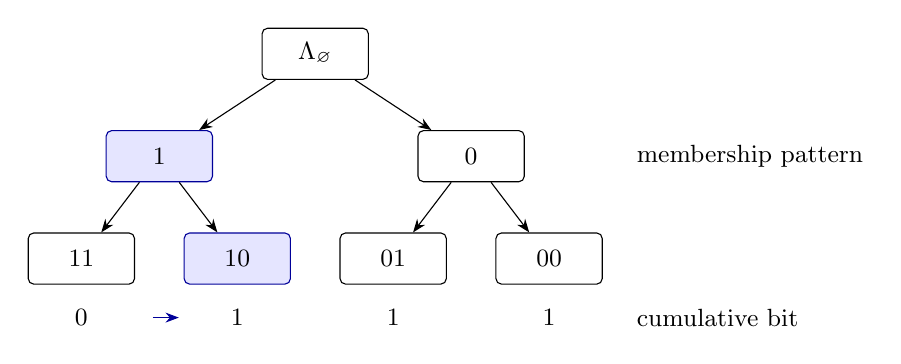
\begin{tikzpicture}[x=1.65cm,y=1cm,>=Stealth,
  cell/.style={draw,rounded corners=2pt,minimum width=1.35cm,
    minimum height=.65cm,font=\small},
  chosen/.style={cell,fill=blue!10,draw=blue!60!black}]
\node[cell] (root) at (0,2.6) {$\Lambda_{\varnothing}$};
\node[chosen] (one) at (-1.2,1.3) {$1$};
\node[cell] (zero) at (1.2,1.3) {$0$};
\node[cell] (oo) at (-1.8,0) {$11$};
\node[chosen] (oz) at (-.6,0) {$10$};
\node[cell] (zo) at (.6,0) {$01$};
\node[cell] (zz) at (1.8,0) {$00$};
\foreach \a/\b in {root/one,root/zero,one/oo,one/oz,zero/zo,zero/zz}
  \draw[->] (\a)--(\b);
\node[font=\small,anchor=west] at (2.4,1.3) {membership pattern};
\node[font=\small,anchor=west] at (2.4,-.75) {cumulative bit};
\foreach \x/\b in {-1.8/0,-.6/1,.6/1,1.8/1}
  \node[font=\small] at (\x,-.75) {$\b$};
\draw[->,blue!60!black] (-1.25,-.75)--(-1.05,-.75);
\end{tikzpicture}
\caption{Schematic transition refinement for two prefix slots. Membership
$1$ precedes $0$ lexicographically. In the illustrated case the cumulative
bit changes at cell $10$, so the transition is in the first cell at depth
one and its second child at depth two. The selected membership bits are
therefore $f_{u_1,\mathcal D_0}(P_1)=1$ and $f_{u_2,\mathcal D_1}(P_2)=0$, with each function using
its preceding prefix. Empty cells are retained in the ordering but cannot
contain a transition.}
\label{fig:prefix-refinement}
\end{figure}


The lemma uses formal product alphabets and literal prefix-lift
identities.  It does not require distinct game vertices in the
prefix.  In particular, a repeated vertex still occupies a
separate slot, with its own independently sampled index and
membership set.

\begin{proposition}[Average acceptance at every scale]
\label{prop:prefix-lower-bound}
Under the common law of $(\mathcal D,e)$, for every $i\in[M]$,
\begin{equation}
  \E h_u(p_i)\ge\frac{p_i}{4}.
  \label{eq:prefix-lower-bound}
\end{equation}
\end{proposition}

\begin{proof}
Consider the full-prefix experiment in
Definition~\ref{def:tests}, with data of length $T$ and an
independent embedding.  Denote its probability and expectation
by $\Pr_{\mathrm{full}}$ and $\E_{\mathrm{full}}$.
Let $Z_T$ be the star set of its wildcard test vertex, and let
$\mathcal A$ be the event that $\mathbf s_T$ is good and its
transition cell is not starred.

The star predicate is constant on each full cell: all label
tuples in that cell have the same membership vector, and hence
the same counts at each scale.  Suppose that $\mathbf s_T$ is
good and its transition cell is starred.  At the cut immediately
before that cell, put
\[
  E=C^{(T)}_{<\tau_T}\setminus Z_T.
\]
This is precisely the union of the nonstar portions of the cells
before the cut.  It is contained in $C^{(T)}_{<\tau_T}$, whose
bit is $0$.  Moreover, $E\cup Z_T$ contains
$C^{(T)}_{\le\tau_T}$, whose bit is $1$: adjoining the stars
restores every earlier starred cell and includes the entire
starred transition cell.  Monotonicity gives
\[
  g_{\mathbf s_T}(E)=0,
  \qquad g_{\mathbf s_T}(E\cup Z_T)=1.
\]
Lemma~\ref{lem:wildcard-forcing} forces deletion of this test
vertex.

The full-prefix family has total mass $H$, so its deletion
probability is at most $D/H$.  The full tuple is independent of
the embedding, and Lemma~\ref{lem:goodness} bounds its badness
probability by $\rho$.  We conclude that
\begin{equation}
  \Pr_{\mathrm{full}}(\mathcal A)
  \ge 1-\rho-\frac{D}{H}
  \ge\frac12.
  \label{eq:full-prefix-favorable}
\end{equation}
The last inequality follows from the parameter choices:
$\rho\le\gamma\le1/4000$ and $D/H<1/8$.

Define $\mathcal D_{j-1}$ from this experiment as in
Lemma~\ref{lem:prefix-refinement}.  For a fixed $i\in[M]$, set
\[
  Y_i=\sum_{j=1}^T
    \ind{i_j=i}\,
    f_{u_j,\mathcal D_{j-1}}(P_j).
\]
On $\mathcal A$, the transition cell is nonstarred, so the
definition of $Z_T$ and
Equation~\eqref{eq:transition-membership} give
$Y_i\ge p_iT/(2M)$.  On all other outcomes, $Y_i\ge0$,
including outcomes for which some conditioned functions use
the fallback rule.  It follows from
Equation~\eqref{eq:full-prefix-favorable} that
\begin{equation}
  \E_{\mathrm{full}}Y_i\ge\frac{p_iT}{4M}.
  \label{eq:full-prefix-count-lower}
\end{equation}

We now calculate this expectation without conditioning on
$\mathcal A$.  For each $j$, condition on the embedding, the
first $j-1$ prefix slots with all their data, and the new
vertex $u_j$.  The function
$f_{u_j,\mathcal D_{j-1}}$ is determined by these choices:
both the goodness test for $\mathbf s_j$ and any fallback
choice are independent of the fresh $i_j$ and $P_j$.
Since $i_j$ is uniform in $[M]$ and $P_j$ has law
$\mu_{p_i}^X$ conditional on $i_j=i$,
\[
  \E_{\mathrm{full}}\!\left[
    \ind{i_j=i} f_{u_j,\mathcal D_{j-1}}(P_j)
    \,\middle|\,
    \psi,(u_\ell,i_\ell,P_\ell)_{\ell<j},u_j
  \right]
  =\frac1M h_{u_j,\mathcal D_{j-1}}(p_i).
\]
The marginal law of the conditioning data and $u_j$ is the
common law of $(\mathcal D,u)$ conditional on $t=j-1$.
Indeed, the new vertex has law $\nu_U$ independently of
the earlier slots, just as does the big endpoint of the
independently sampled edge.  Therefore
\begin{align*}
  \E_{\mathrm{full}}Y_i
  &=\frac1M\sum_{j=1}^T
      \E\bigl[h_u(p_i)\mid t=j-1\bigr]\\
  &=\frac TM\E h_u(p_i).
\end{align*}
Together with Equation~\eqref{eq:full-prefix-count-lower},
this proves Equation~\eqref{eq:prefix-lower-bound}.
\end{proof}

The shared distribution in
Equation~\eqref{eq:common-conditioning} has not changed with
$i$.  The favorable full-chain event was used only to bound
a nonnegative random sum from below; it was not used to
condition the expectation that identifies this sum with
$\E h_u(p_i)$.

\section{A budget for pivotal labels}
\label{sec:pivotality}

We associate to each conditioned function a quantity that controls both its
influences and its acceptance probabilities at every bias.  The single-label
tests bound the expectation of this quantity under the common distribution
from Section~\ref{sec:prefix}.
A single test vertex may have several cuts that force its deletion, but its
cost is paid only once.  Accordingly, we record whether a label is pivotal
somewhere along a permutation, rather than the number of witnessing prefixes.

\begin{definition}[Pivotality budget]
\label{def:pivotal-budget}
Let $S$ be a nonempty finite set, and let
$f:2^S\to\{0,1\}$ be monotone with $f(\varnothing)=0$ and $f(S)=1$.
For each $j\in S$, let $\sigma_j$ be a uniform permutation of
$S\setminus\{j\}$.  Write $R_a(\sigma_j)$ for the set of its first $a$
elements, where $0\le a\le |S|-1$.  Define
\[
 B(f)=\sum_{j\in S}
 \Pr_{\sigma_j}\!\left[
 \begin{gathered}
   \text{there exists }a\in\{0,\ldots,|S|-1\}\text{ such that}\\
   f(R_a(\sigma_j))=0,\quad
   f(R_a(\sigma_j)\cup\{j\})=1
 \end{gathered}
 \right].
\]
Thus both the empty prefix and the full prefix $S\setminus\{j\}$ are
allowed.  A permutation contributes only once for a given $j$, even when
several of its prefixes witness pivotality.  In particular,
$0\le B(f)\le |S|$.
\end{definition}

\begin{lemma}[Arrival-time inequalities]
\label{lem:pivotal-inequalities}
For every function in Definition~\ref{def:pivotal-budget} and every
$0<p<1$,
\[
 I_p(f)\le B(f),
 \qquad
 \mathbb E_{R\sim\mu_p^S} f(R)\le pB(f).
\]
\end{lemma}

\begin{proof}
Give each $j\in S$ an independent uniform arrival time $T_j\in[0,1]$.
With probability one all these times are distinct.  For each $j$, let
$\sigma_j$ be the order in which the other elements arrive, and let
$\mathcal A_j$ be the event that some prefix of $\sigma_j$ witnesses
$j$'s pivotality in Definition~\ref{def:pivotal-budget}.  The permutation
$\sigma_j$ is uniform, so
\[
 \sum_{j\in S}\Pr(\mathcal A_j)=B(f).
\]
Moreover, $\mathcal A_j$ is determined entirely by the arrival times of
elements other than $j$, and hence is independent of $T_j$.

For the influence inequality, put
\[
 R_{-j}(p)=\{k\in S\setminus\{j\}:T_k\le p\}.
\]
This set has law $\mu_p^{S\setminus\{j\}}$ and is a prefix of
$\sigma_j$.  By monotonicity, the event defining $I_{p,j}(f)$ is exactly
\[
 \{f(R_{-j}(p))=0,\ f(R_{-j}(p)\cup\{j\})=1\},
\]
which is contained in $\mathcal A_j$.  Summing
$I_{p,j}(f)\le\Pr(\mathcal A_j)$ over $j$ proves $I_p(f)\le B(f)$.

For the acceptance inequality, put $R(p)=\{j\in S:T_j\le p\}$, which
has law $\mu_p^S$.  Along the complete arrival sequence, the value of
$f$ starts at zero, ends at one, and never decreases.  There is therefore
a unique arriving element at which it changes from zero to one.  If
$f(R(p))=1$ and this element is $j$, then $T_j\le p$, and the elements
arriving before $j$ form a prefix of $\sigma_j$ witnessing
$\mathcal A_j$.  Consequently, up to the null event of tied arrival times,
\[
 \{f(R(p))=1\}
 \subseteq\bigcup_{j\in S}\bigl(\{T_j\le p\}\cap\mathcal A_j\bigr).
\]
A union bound and the independence established above give
\[
 \mathbb E_{R\sim\mu_p^S} f(R)
 \le\sum_{j\in S}\Pr(T_j\le p,\mathcal A_j)
 =p\sum_{j\in S}\Pr(\mathcal A_j)
 =pB(f).
\]
Only the possible-witness event $\mathcal A_j$ is asserted to be
independent of $T_j$; no independence of the actual switching element is
needed.
\end{proof}

Return to the fixed feedback vertex set $F$ of cost at most $D$ and its
fixed topological order.  For the functions in
Definition~\ref{def:conditioned-functions}, set
\[
 B_w=B(f_w)\qquad(w\in U\cup V).
\]
These variables depend on the shared data $\mathcal D$ and the named
vertex $w$.  Their definition does not involve a fresh tested edge or a
fresh bias index.  Lemma~\ref{lem:pivotal-inequalities} gives, for every
realization of these data and every $0<p<1$,
\[
 I_p(f_w)\le B_w,
 \qquad h_w(p)\le pB_w.
\]

\begin{proposition}[Single-label test budget]
\label{prop:pivotal-budget}
Under the common law of $\mathcal D$ and an independent edge
$e=(u,v)\sim\nu$,
\begin{equation}
 \mathbb E B_u\le D+1,
 \qquad
 \mathbb E B_v\le D+1.
 \label{eq:pivotal-budget}
\end{equation}
\end{proposition}

\begin{proof}
Fix either side of the game and sample $w$ independently of
$\mathcal D$ from that side's endpoint marginal.  Its alphabet size
$m_w$ is constant on the chosen side.  This is exactly the marginal law
of the shared data and endpoint in the corresponding single-label test
family of Definition~\ref{def:tests}.

First fix $\mathcal D,w$ for which the extension $\mathbf s w$ is good.
The conditioned function $f_w$ then uses the transition cell $C_{r_*}$.
The remaining randomness of a single-label test consists of a uniform
label $j_0\in\Lambda_w$ and an independent uniform permutation $\sigma$
of $\Lambda_w$.  Its star set is
\[
 Z=\Lambda_{\mathbf s}\times\{j_0\},
\]
and its ordered cells are $C_\ell\times\{j\}$, first ordered by
$\ell$ and then by $\sigma$.  Suppose some prefix $R$ of $\sigma$ with
$j_0$ omitted satisfies
\[
 f_w(R)=0,
 \qquad f_w(R\cup\{j_0\})=1.
\]

Choose a cut among the refined cells belonging to $C_{r_*}$, including
either boundary of this block if necessary, so that precisely the
nonstar labels in $R$ have been passed within that block.  Such a cut
exists because deleting $j_0$ from the sequence $\sigma$ preserves the
order of every other label.  For $R=\varnothing$ one may cut before the
block, and for $R=\Lambda_w\setminus\{j_0\}$ one may cut after the
block.  Let $E$ be the union of all refined cells before the cut, with
all stars removed.  Then exactly
\[
 E=\bigl((C_{<r_*}\times\Lambda_w)\setminus Z\bigr)
       \cup(C_{r_*}\times R).
\]
In particular,
\[
 E\subseteq E_w^{r_*}(R),
 \qquad
 E\cup Z\supseteq E_w^{r_*}(R\cup\{j_0\}).
\]
The second inclusion restores the stars in all earlier prefix cells;
the additional stars in later cells only enlarge the set.  Monotonicity
of $g_{\mathbf s w}$ and the definition of $f_w$ now imply
\[
 g_{\mathbf s w}(E)=0,
 \qquad g_{\mathbf s w}(E\cup Z)=1.
\]
Lemma~\ref{lem:wildcard-forcing} therefore forces this test vertex to
belong to $F$.

This argument uses the ordered partition with its empty cells retained;
the set identities remain valid when some of those cells are empty.
They also hold on the formal product label domain when $w$ or another
game vertex occurs repeatedly in the tuple.  No independence of labels
in repeated slots is assumed, and the use of $f_w$ rests only on the
prefix identifications of Lemma~\ref{lem:compatibility}.

For each fixed $j_0$, deleting $j_0$ from a uniform permutation of
$\Lambda_w$ gives a uniform permutation of
$\Lambda_w\setminus\{j_0\}$.  Averaging the forced-deletion event over
the uniform choice of $j_0$ therefore gives, whenever $\mathbf s w$ is
good,
\[
 \Pr[\text{sampled test vertex}\in F\mid\mathcal D,w]
 \ge \frac{B_w}{m_w}.
\]
Here a test is charged once if a witnessing prefix exists, regardless
of how many prefixes witness the same label's pivotality.

Let $\mathcal G_w$ denote the event that $\mathbf s w$ is good.
The total mass of the chosen test family is $m_w$, and its vertices
carry their sampling probabilities times this mass.  Thus, on taking
expectations, the cost spent by $F$ in this family is at least
$\mathbb E[B_w\mathbf 1_{\mathcal G_w}]$.  Since the total cost of
$F$ is at most $D$,
\[
 \mathbb E[B_w\mathbf 1_{\mathcal G_w}]\le D.
\]
On the complementary event the fallback function is still monotone,
with bottom zero and top one, so Definition~\ref{def:pivotal-budget}
gives $B_w\le m_w$.  The sampled-extension bound from
Equation~\eqref{eq:sampled-extension-bad} gives
$\Pr(\mathcal G_w^c)\le\rho$; equivalently, one may apply
Lemma~\ref{lem:goodness} after fixing the sampled vertex tuple, which
is independent of $\psi$.  As $m_w\le m$ and $\rho\le1/m$,
\[
 \mathbb E[B_w\mathbf 1_{\mathcal G_w^c}]
 \le m_w\rho\le1.
\]
Adding the two bounds proves $\mathbb E B_w\le D+1$ for either
endpoint marginal, and hence proves Equation~\eqref{eq:pivotal-budget}.
\end{proof}

\section{Soundness from coupled comparisons}
\label{sec:soundness}

Assume that the game has value at most \(\theta\), and suppose that
the constructed digraph has a feedback vertex set \(F\) of cost at
most \(D\).  Continue with the fixed topological order \(\prec\)
and the conditioned functions from Sections~\ref{sec:ranks}
and~\ref{sec:prefix}.  In particular, \(\mathcal D\) denotes the
shared data in Equation~\eqref{eq:common-conditioning}, and a fresh
edge \(e=(u,v)\) has law \(\nu\) independently of \(\mathcal D\).
The random variables \(f_w,h_w(p)\), and \(B_w=B(f_w)\) are defined
for every vertex \(w\) once \(\mathcal D\) is fixed.

For a fixed \(i\in[M]\), there are two experiments for the fresh
subsets at the sampled edge.  In the \emph{coupled experiment},
\((R_u,R_v)\) has the law of the comparison test at index \(i\).
In the \emph{independent experiment}, conditionally on
\((\mathcal D,e)\), the subsets are independent with laws
\(\mu_{p_i}^{X}\) and \(\mu_{q_i}^{Y}\).
We write \(\Pr_{\mathrm c,i}\) and \(\Pr_{\mathrm{ind},i}\) for
probabilities in these experiments, including the common law of
\((\mathcal D,e)\).  Neither experiment samples a candidate cell
unless this is explicitly stated.

\subsection{Coupling and deletion cost}

Recall the coupling from the comparison family in
Definition~\ref{def:tests}.  For \(p=p_i\le1/4\), its exact
marginals are \(\mu_p^X\) and \(\mu_{2p}^Y\), and
Equation~\eqref{eq:coupling-inclusion} gives
\[
  R_u\subseteq\pi_e^{-1}(R_v)
  \quad\hbox{in every coupled outcome.}
\]
For each \(y\in Y\), the block consists of the two bits in
\(\pi_e^{-1}(y)\) and the bit at \(y\).  These blocks are
independent across \(y\).  The marginals and block independence
hold for every fixed edge, independently of the shared prefix data.

\begin{lemma}[Comparison deletion charge]
\label{lem:comparison-charge}
For every \(i\in[M]\),
\begin{equation}
\label{eq:coupled-comparison}
  \Pr_{\mathrm c,i}[\,f_u(R_u)=1,\ f_v(R_v)=0\,]
    \le 2\rho+\frac{M2^T D}{K}.
\end{equation}
\end{lemma}

\begin{proof}
Let \(\mathcal G\) be the event that both extended tuples
\(\mathbf s u\) and \(\mathbf s v\) are good.  The tuple choices
are independent of \(\psi\), so Lemma~\ref{lem:goodness}, averaged
over these choices, gives \(\Pr[\mathcal G^c]\le2\rho\).
On \(\mathcal G\), both conditioned functions use the same prefix
transition index \(r_*\), by Definition~\ref{def:conditioned-functions}
and Lemma~\ref{lem:compatibility}.

Suppose that \(\mathcal G\) holds and that
\(f_u(R_u)=1,\ f_v(R_v)=0\).  Add the candidate-cell draw from
the comparison test and consider the outcome \(r=r_*\).
The start and end rank vertices of Equation~\eqref{eq:comparison-path}
are then
\[
  b_{\mathbf s v}^{\psi}
      (E_v^{r_*}(R_v);2,17),
  \qquad
  b_{\mathbf s u}^{\psi}
      (E_u^{r_*}(R_u);3,18).
\]
The triples \((2,15,17)\) and \((3,15,18)\) are usable.
Goodness and the two function values show that the start does not
precede \(o_{\psi(15)}\), whereas the end precedes \(o_{\psi(15)}\).
If the test vertex were retained, its two arcs would require the
start to precede the test vertex and the test vertex to precede the
end.  This contradicts the fixed topological order.  Hence that
comparison vertex belongs to \(F\).

For fixed \((\mathcal D,e,R_u,R_v)\) as above, the candidate-cell
draw hits \(r_*\) with probability \(2^{-t}\ge2^{-T}\).
Let \(\delta_i\) be the probability that a comparison vertex is
deleted when its fresh threshold index is fixed to \(i\), including
the candidate-cell draw.  We have proved
\[
  \delta_i\ge
   2^{-T}\Pr_{\mathrm c,i}
     [\,\mathcal G,\ f_u(R_u)=1,\ f_v(R_v)=0\,].
\]
In the actual comparison family the threshold index is uniform on
\([M]\).  Its deleted weight is
\[
  \frac K M\sum_{j=1}^{M}\delta_j\le D,
\]
so \(\delta_i\le MD/K\).
Combining these inequalities and then adding
\(\Pr[\mathcal G^c]\le2\rho\) proves
Equation~\eqref{eq:coupled-comparison}.
\end{proof}

\subsection{Lists chosen before the edge}

\begin{lemma}[List decoding against game soundness]
\label{lem:list-decoding}
Suppose a game has value at most \(\theta\).
Assign to every game vertex \(w\) a list
\(J_w\subseteq\Lambda_w\), possibly empty, of cardinality at most
an integer \(J\ge1\).  Then
\[
  \Pr_{e=(u,v)\sim\nu}
    [\,\pi_e(J_u)\cap J_v\ne\varnothing\,]\le\theta J^2.
\]
The same conclusion holds conditionally on any data independent of
the fresh edge, if all the lists are fixed by those data.
\end{lemma}

\begin{proof}
Independently for each vertex with a nonempty list, choose its label
uniformly from that list.  Give every empty-list vertex any fixed
label from its alphabet.  If
\(\pi_e(J_u)\cap J_v\ne\varnothing\), there is at least one pair
\((x,y)\in J_u\times J_v\) with \(\pi_e(x)=y\).  Since \(u\) and
\(v\) are different vertices, the probability of choosing that pair
is
\[
  \frac1{\abs{J_u}\abs{J_v}}\ge\frac1{J^2}.
\]
The expected value of this random labeling is therefore at least
the displayed intersection probability divided by \(J^2\).
Every deterministic labeling in its support has value at most
\(\theta\), so the expected value is at most \(\theta\).
This proves the claim.  For the conditional assertion, fix the
conditioning data first and repeat the same argument; independence
leaves the fresh edge law equal to \(\nu\).
\end{proof}

\subsection{Replacing the coupling by product measure}

\begin{proposition}[Product comparison]
\label{prop:product-comparison}
For every \(i\in[M]\), under the common distribution of
\((\mathcal D,e)\),
\begin{equation}
\label{eq:product-comparison}
  \E\bigl[h_u(p_i)(1-h_v(q_i))\bigr]\le\frac{p_i}{16}.
\end{equation}
\end{proposition}

\begin{proof}
Fix \(i\).  For each value of \(\mathcal D\), construct a junta
approximant for each game vertex, before drawing the fresh edge.
For notation, put
\[
  \beta_{w,i}=
  \begin{cases}
    p_i,&w\in U,\\
    q_i,&w\in V.
  \end{cases}
\]
If \(B_w\le B_0\), Lemma~\ref{lem:pivotal-inequalities} gives
\(I_{\beta_{w,i}}(f_w)\le B_0\).
Corollary~\ref{cor:dyadic-junta} and the choice of \(J\) in
Section~\ref{sec:parameters} therefore provide a Boolean function
\(\widetilde f_{w,i}\) on a coordinate set
\(J_w\subseteq\Lambda_w\), with
\begin{equation}
\label{eq:junta-error}
  \abs{J_w}\le J,\qquad
  \Pr_{R\sim\mu_{\beta_{w,i}}^{\Lambda_w}}
    [\,f_w(R)\ne\widetilde f_{w,i}(R)\,]\le\gamma.
\end{equation}
Choose one such pair by a fixed ordering of the finitely many
possible coordinate sets and Boolean truth tables.
If \(B_w>B_0\), set \(J_w=\varnothing\) and choose
\(\widetilde f_{w,i}\) to be the constant-zero function; no error
guarantee is asserted at that vertex.
We suppress the dependence of \(J_w\) on \(\mathcal D\) and \(i\).

This defines one list for every actual game vertex from
\((\mathcal D,i)\) alone.  The functions \(f_w\), including the
fallback functions, are already defined for all vertices from
\(\mathcal D\) alone.  Thus the choice of a junta or list uses no
information about the fresh sampled edge.  It may depend on the
fixed game instance and the fixed topological order, as may any
labeling used in a soundness argument.  A repetition in the prefix,
or an endpoint that also occurs in the prefix, does not change this
conditional independence: the fresh edge was drawn independently
of the entire prefix.

By Lemma~\ref{lem:list-decoding}, for every fixed value of
\(\mathcal D\),
\[
  \Pr_{e\sim\nu}
     [\,\pi_e(J_u)\cap J_v\ne\varnothing
        \mid\mathcal D\,]\le\theta J^2.
\]
After averaging over \(\mathcal D\), this remains the bound on the
list-intersection event under the common law.
Also, Proposition~\ref{prop:pivotal-budget} and Markov's
inequality give the averaged bound
\begin{equation}
\label{eq:budget-cutoff}
  \Pr[\,B_u>B_0\ \text{or}\ B_v>B_0\,]
   \le\frac{\E B_u+\E B_v}{B_0}
   \le 2\gamma.
\end{equation}
Here we have used the actual endpoint marginals of \(\nu\).
Equation~\eqref{eq:budget-cutoff} is a bound under the joint law of
\((\mathcal D,e)\); no corresponding pointwise bound conditional
on \(\mathcal D\) is needed.

Let \(\mathcal A_i\) be the event, determined by
\((\mathcal D,e)\), that both budgets are at most \(B_0\) and
\(\pi_e(J_u)\cap J_v=\varnothing\).  The preceding bounds imply
\begin{equation}
\label{eq:junta-exceptions}
  \Pr[\mathcal A_i^c]\le2\gamma+\theta J^2.
\end{equation}
Fix \((\mathcal D,e)\) in \(\mathcal A_i\).
In the coupled experiment, all bits used by the big-side junta
belong to fibers indexed by \(\pi_e(J_u)\), and all bits used by
the small-side junta belong to fibers indexed by \(J_v\).
These are disjoint collections of independently generated fibers.
Consequently
\(\widetilde f_{u,i}(R_u)\) and
\(\widetilde f_{v,i}(R_v)\) are independent in the coupled
experiment.  They are also independent in the independent
experiment, and their marginal distributions are unchanged.
Their joint distributions therefore agree in the two experiments.
This includes the case of a constant junta with an empty
coordinate set.

The conditional approximation error for each endpoint in
Equation~\eqref{eq:junta-error} is at most \(\gamma\) in either
experiment, because both have exactly the stipulated product
marginals.  Replacing \(f_u,f_v\) by their respective juntas changes
the conditional probability of the pattern \((1,0)\) by at most
\(2\gamma\), by a union bound.  Doing this in both experiments and
using equality of the junta joint distributions yields
\begin{align*}
 &\left|
  \Pr_{\mathrm{ind},i}[\,f_u(R_u)=1,\ f_v(R_v)=0
                      \mid\mathcal D,e\,]
 \right.\\[-2mm]
 &\hspace{22mm}\left.
  -\Pr_{\mathrm c,i}[\,f_u(R_u)=1,\ f_v(R_v)=0
                      \mid\mathcal D,e\,]
  \right|\le4\gamma
\end{align*}
on \(\mathcal A_i\).
On its complement the difference is at most one.
Integrating over the unchanged law of \((\mathcal D,e)\), and using
Equation~\eqref{eq:junta-exceptions} and
Lemma~\ref{lem:comparison-charge}, gives
\begin{align}
\label{eq:product-comparison-error}
  &\Pr_{\mathrm{ind},i}[\,f_u(R_u)=1,\ f_v(R_v)=0\,]\notag\\
  &\qquad\le
  2\rho+\frac{M2^T D}{K}
      +2\gamma+\theta J^2+4\gamma
  \le10\gamma.
\end{align}
The conditional probability of the pattern in the independent
experiment is exactly \(h_u(p_i)(1-h_v(q_i))\).
Finally, \(\gamma=p_M/1000\) and \(p_M\le p_i\), so
\[
  10\gamma=\frac{p_M}{100}\le\frac{p_i}{16}.
\]
This proves Equation~\eqref{eq:product-comparison}.
\end{proof}

\subsection{The dyadic tail contradiction}

\begin{proposition}[Weighted soundness]
\label{prop:weighted-soundness}
If the game has value at most \(\theta\), every feedback vertex set
of the constructed weighted digraph has cost strictly greater
than \(D\).
\end{proposition}

\begin{proof}
Suppose that \(F\) has cost at most \(D\), as assumed throughout
this section.  Fix \(i\in[M]\), and let
\[
  \mathcal H_i=\{h_v(q_i)\ge1/2\}
\]
under the common distribution of \((\mathcal D,e)\).
On its complement,
\(h_u(p_i)\le2h_u(p_i)(1-h_v(q_i))\).  Consequently
Propositions~\ref{prop:prefix-lower-bound}
and~\ref{prop:product-comparison} imply
\begin{align*}
  \E[\,h_u(p_i)\ind{\mathcal H_i}\,]
  &=\E h_u(p_i)
       -\E[\,h_u(p_i)\ind{\mathcal H_i^c}\,]\\
  &\ge\frac{p_i}{4}
       -2\E[\,h_u(p_i)(1-h_v(q_i))\,]\\
  &\ge\frac{p_i}{8}.
\end{align*}
Since \(0\le h_u(p_i)\le1\), we obtain
\(\Pr[\mathcal H_i]\ge p_i/8\).
Lemma~\ref{lem:pivotal-inequalities} also gives
\(h_v(q_i)\le q_iB_v=2p_iB_v\) pointwise.
Thus, on \(\mathcal H_i\), one has \(B_v\ge1/(4p_i)\), and hence
\begin{equation}
\label{eq:dyadic-budget-tails}
  \Pr\!\left[B_v\ge\frac1{4p_i}\right]\ge\frac{p_i}{8},
  \qquad i\in[M].
\end{equation}

These are tail estimates for one random variable \(B_v\) under one
fixed probability law.  The definition of \(f_v\), and therefore
that of \(B_v\), does not use the fresh threshold index \(i\).
The junta approximants used to prove the individual estimates may
depend on \(i\), but this does not alter \(B_v\).

Put \(a_i=1/(4p_i)\) for \(i\ge1\), and \(a_0=0\).
For every real \(x\ge0\),
\[
  x\ge\sum_{i=1}^{M}(a_i-a_{i-1})\ind{x\ge a_i}.
\]
Indeed, if \(a_j\) is the largest crossed threshold, the sum on the
right telescopes to \(a_j\le x\); if no threshold is crossed, it
is zero.  Taking expectations and using
Equation~\eqref{eq:dyadic-budget-tails} yields
\[
  \E B_v
  \ge\sum_{i=1}^{M}(a_i-a_{i-1})\Pr[B_v\ge a_i]
  \ge\sum_{i=1}^{M}\frac{a_i}{2}\frac{p_i}{8}
  =\frac M{64}.
\]
Here \(a_i=2a_{i-1}\) for \(i\ge2\), while
\(a_1-a_0=a_1\ge a_1/2\).
Since \(M=128(D+1)\), this gives
\(\E B_v\ge2(D+1)\), contradicting
Proposition~\ref{prop:pivotal-budget}.
No feedback vertex set of cost at most \(D\) can therefore exist.
\end{proof}

\section{Removing the vertex costs}
\label{sec:unweighting}

The weighted gap converts to an unweighted gap without requiring a common
denominator for all vertex costs.  Rounding upward at a scale determined
by the number of vertices controls the additive loss. Independent-copy
blowups also occur in earlier DFVS hardness reductions
\cite[Section~2]{GuruswamiLee2016}. The rounding below allows arbitrary
rational costs of polynomial bit length without expanding a common
denominator.

\begin{lemma}[Rounding and cloning]
\label{lem:round-and-clone}
Let $G$ be a loopless digraph on $S\ge1$ vertices with positive rational
vertex costs $w_v\le C$.  Set $c_v=\lceil Sw_v\rceil$.  Replace every vertex
$v$ by an independent set $\mathcal C_v$ of $c_v$ unweighted vertices, and
replace every arc $u\to v$ by all arcs from $\mathcal C_u$ to
$\mathcal C_v$.  Call the resulting digraph $\widehat G$.  Then
\begin{equation}
  \DFVS(\widehat G)
  =\min\left\{\sum_{v\in F}c_v:
      F\text{ is a feedback vertex set of }G\right\}.
  \label{eq:clone-exact-optimum}
\end{equation}
The number of vertices of $\widehat G$ is at most $CS^2+S$.  For fixed
$C$, this is a deterministic polynomial construction in the encoding size
of $G$ and its costs.  Moreover:
\begin{enumerate}[label=(\roman*)]
  \item a feedback vertex set of $G$ of cost at most $a$ yields a feedback
  vertex set of $\widehat G$ of size at most $S(a+1)$;
  \item if every feedback vertex set of $G$ has cost greater than $b$,
  then $\DFVS(\widehat G)>Sb$.
\end{enumerate}
\end{lemma}

\begin{proof}
Let $F$ be a feedback vertex set of $G$.  Deleting every cluster
$\mathcal C_v$ with $v\in F$ leaves only clusters over the acyclic digraph
$G-F$.  Lift a topological order of $G-F$ by placing all vertices of each
cluster consecutively.  Since clusters are independent, this is a
topological order of the surviving vertices of $\widehat G$.  It gives a
feedback vertex set of size $\sum_{v\in F}c_v$.

Conversely, let $Q$ be any feedback vertex set of $\widehat G$, and define
\[
  F_Q=\{v\in V(G):\mathcal C_v\subseteq Q\}.
\]
If $G-F_Q$ contained a directed cycle, every cluster over that cycle would
contain a surviving vertex.  Choosing one such vertex from each cluster
would lift the original cycle to a directed cycle of $\widehat G-Q$,
because all the intercluster arcs in the requisite directions are present.
This is impossible.  Thus $F_Q$ is a feedback vertex set of $G$, and
\[
  \sum_{v\in F_Q}c_v\le\abs{Q}.
\]
Together with the preceding construction, this proves
Equation~\eqref{eq:clone-exact-optimum}.  In particular, partial deletions
from a cluster cannot improve the optimum beyond the corresponding
choice of completely deleted clusters.

For every $v$ we have
\[
  Sw_v\le c_v<Sw_v+1.
\]
Summing over any feedback vertex set $F$ gives
\[
  S\sum_{v\in F}w_v
  \le\sum_{v\in F}c_v
  \le S\sum_{v\in F}w_v+S.
\]
This proves both gap implications by
Equation~\eqref{eq:clone-exact-optimum}.  Equivalently, the rounded costs
$c_v/S$ increase the cost of any deletion set by at most one.

Finally,
\[
  \abs{V(\widehat G)}=\sum_vc_v\le CS^2+S.
\]
There are at most the square of this number of arcs.  Each $c_v$ is
computed exactly by integer arithmetic on the rational input cost.
For fixed $C$, the vertices and arcs can therefore be listed in
polynomial time.  Positivity of the costs ensures that every cluster is
nonempty before deletions.  The assumption that $G$ is loopless ensures
that independent clusters realize precisely the prescribed construction.
\end{proof}

\begin{remark}[Avoiding opposite arcs]
\label{rem:no-opposite-arcs}
The construction above already gives loopless digraphs, and unrestricted
DFVS permits opposite arcs.  If opposite arcs are to be excluded, subdivide
every weighted arc using a distinct private vertex of cost $D+1$ before
applying Lemma~\ref{lem:round-and-clone}.  A feedback vertex set of cost at
most $4$ in the original graph still works in the subdivided graph: a
cycle avoiding that set would project to a directed closed walk, hence
to a directed cycle, in the original remaining graph.  On the other hand,
a deletion set of cost at most $D$ cannot contain any subdivision vertex.
Every surviving original cycle would then lift through its private
subdivisions, so the weighted soundness bound is preserved as well.
Subdivision of every arc of a loopless digraph leaves no pair of opposite
arcs, and the subsequent independent-cluster construction preserves this
property.  The additional vertices have constant cost and polynomial
number, so the size bounds needed for rounding remain valid.
\end{remark}

\begin{proof}[Proof of Theorem~\ref{thm:main}]
It suffices to prove the claim for every fixed integer $A\ge1$: given any
fixed real factor, choose an integer at least as large.  For this integer
$A$, choose the parameters of Section~\ref{sec:parameters} and start from
the NP-hard promise problem of Theorem~\ref{thm:games} at the resulting
fixed $\theta$.

By Proposition~\ref{prop:polynomial}, the weighted reduction is
deterministic and polynomial in the game input size, and all its costs are
bounded by the constant $C_A$.  Proposition~\ref{prop:completeness} gives
a feedback vertex set of cost at most $4$ in the YES case, while
Proposition~\ref{prop:weighted-soundness} shows that every feedback vertex
set has cost greater than $D=10A$ in the NO case.  Let $S$ be the number of
weighted vertices.  Lemma~\ref{lem:round-and-clone} gives an unweighted
digraph $\widehat G$ with the gap
\[
  \begin{array}{ll}
    \text{YES:}&\DFVS(\widehat G)\le5S,\\[2pt]
    \text{NO:}&\DFVS(\widehat G)>DS.
  \end{array}
\]
This last transformation is polynomial because $C_A$ is fixed.  Set
$k=5S$ and output the pair $(\widehat G,k)$.  In the YES case,
$\DFVS(\widehat G)\le k$, whereas in the NO case
\[
  \DFVS(\widehat G)>DS=10AS>5AS=Ak.
\]
Thus this pair has the promised gap of Theorem~\ref{thm:main}.

A deterministic polynomial-time $A$-approximation would return a feasible
feedback vertex set of size at most $5AS<DS$ on every YES instance.  On a
NO instance, every feasible feedback vertex set has size greater than
$DS$.  Comparing the returned size with the known threshold $DS$ would
therefore distinguish the NP-hard promise cases in polynomial time.
This proves the asserted NP-hardness for every fixed constant factor,
and its deterministic consequence under $\mathrm P\ne\mathrm{NP}$.
\end{proof}


A \emph{directed feedback arc set} is a set of arcs whose deletion leaves
an acyclic digraph.  Write $\operatorname{DFAS}(H)$ for its minimum
cardinality.

\begin{corollary}[Directed feedback arc set]
\label{cor:feedback-arc}
For every fixed real $A\ge1$, approximating directed feedback arc set
within factor $A$ is NP-hard on unweighted simple loopless digraphs.
More precisely, there is a deterministic polynomial reduction producing
such a digraph $H$ and a positive integer $k$ with the promise gap
\[
  \begin{array}{ll}
    \text{YES:}&\operatorname{DFAS}(H)\le k,\\[2pt]
    \text{NO:}&\operatorname{DFAS}(H)>Ak.
  \end{array}
\]
\end{corollary}

\begin{proof}
Let $G=(V,E)$ be an unweighted loopless digraph, with $n=\abs{V}$ and
$m=\abs{E}$.  Split each vertex $v$ into $v^-,v^+$ and insert the arc
$a_v:v^-\to v^+$.  For every original arc $e=(u,v)$, introduce $n+1$
fresh private vertices $w_{e,j}$ and the paths
\[
  u^+\longrightarrow w_{e,j}\longrightarrow v^-\qquad(1\le j\le n+1).
\]
Call the resulting unweighted digraph $H$.  All private vertices are
distinct, so $H$ has no loops or repeated arcs, even if $G$ has opposite
arcs.  It has $2n+(n+1)m$ vertices and $n+2(n+1)m$ arcs and is explicitly
constructible in polynomial time.

If $S$ is a feedback vertex set of $G$, deleting the arcs $a_v$ for
$v\in S$ destroys every directed cycle of $H$: a surviving cycle would
alternate distinguished arcs with connector paths and project to a
directed closed walk in $G-S$.  Hence
$\operatorname{DFAS}(H)\le\DFVS(G)\le n$.

Conversely, let $F$ be any feedback arc set of $H$.  If $\abs{F}\ge n$,
return $S=V$, which is a feedback vertex set of size at most $\abs{F}$.
If $\abs{F}<n$, return $S=\{v:a_v\in F\}$, again of size at most
$\abs{F}$.  Were there a directed cycle in $G-S$, every distinguished arc
needed to lift it would survive.  For each original arc of the cycle,
its $n+1$ connector paths are pairwise edge-disjoint, so at least one
survives deletion of $F$.  Choosing these paths would lift the cycle to
$H-F$, a contradiction.  Thus the returned $S$ is always a feedback
vertex set, and this recovery is polynomial time.

The two maps give $\operatorname{DFAS}(H)=\DFVS(G)$.  They also preserve
approximation solutions: an $A$-approximate $F$ yields
$\abs{S}\le\abs{F}\le A\operatorname{DFAS}(H)=A\DFVS(G)$.
Composing this construction with Theorem~\ref{thm:main} and retaining its
positive integer threshold $k$ proves the stated gap.
\end{proof}

\bibliographystyle{plain}
\par
\begingroup
\small
\bibliography{references}
\endgroup
\end{document}
